%% This is an example first chapter.  You should put chapter/appendix that you
%% write into a separate file, and add a line \include{yourfilename} to
%% main.tex, where `yourfilename.tex' is the name of the chapter/appendix file.
%% You can process specific files by typing their names in at the 
%% \files=
%% prompt when you run the file main.tex through LaTeX.
\chapter{Nonlinear Aircraft Model}

The movement of any object can be represented by changes in its location (translation) or changes in its attitude (rotation) or a combination of both. 
Motion of an aircraft is usually involves both translation and rotation. 
Studying aircraft motion is complicated since those two motions are coupled, e.g a rotation might cause a change in aerodynamic forces which affects the translation. 
Thus, to ease the process the motion is broken into easier problems utilizing some assumptions. 
Such an assumption for the aircraft motion is to assume that the aircraft is a point mass, all its mass collected at its center of gravity, so translates from one point to the other. 
Then, the aircraft's rotation is investigated by no longer assuming it as a point mass but a rigid body in space.
In this chapter, modeling both of these motions have been presented in detail.
  
\section{Attitude motion modeling}

Rotation is a change in an object's attitude. 
A change in attitude is modeled using rotations about the center of gravity.  
This section derives the equations for rotation (attitude motion).

Rotations are directly affected by external torques and moments while translations are directly affected external forces. 
Also, attitude of an aircraft during translation affects the aerodynamic forces causing an change in translation.

A force applied at a distance from the center of mass causes a rotation.
A very common approach during aircraft control studies is to balance those rotations, by trimming the aircraft, such that the aircraft will not rotate.

In this section, attitude motion is represented with kinematic and dynamics equations. 
First different parametrization of attitude, such as euler angles and quaternions, are discussed. 
Then kinematic and dynamic equations of attitude motion are derived for a general rigid body. 
These equations are later specified for the aircraft as the rigid body of interest. 

\subsection{Attitude representations}
Let us say triad $b_1, b_2, b_3$ of unit vectors representing an orthogonal coordinate system is attached to a rigid body, such that

\begin{equation}
\label{eqn:unitVectors}
\bm{b_1}\times \bm{b_2}= \bm{b_3}
\end{equation}

The rigid body is composed of points, which do not experience any distance change in between during motion of the body. 
Problem of representing attitude can simply be thought of specifying the orientation of this triad with respect to some reference frame A such as in Fig.~\ref{fig:theTwoFrames}.

\begin{figure}
\begin{center}
%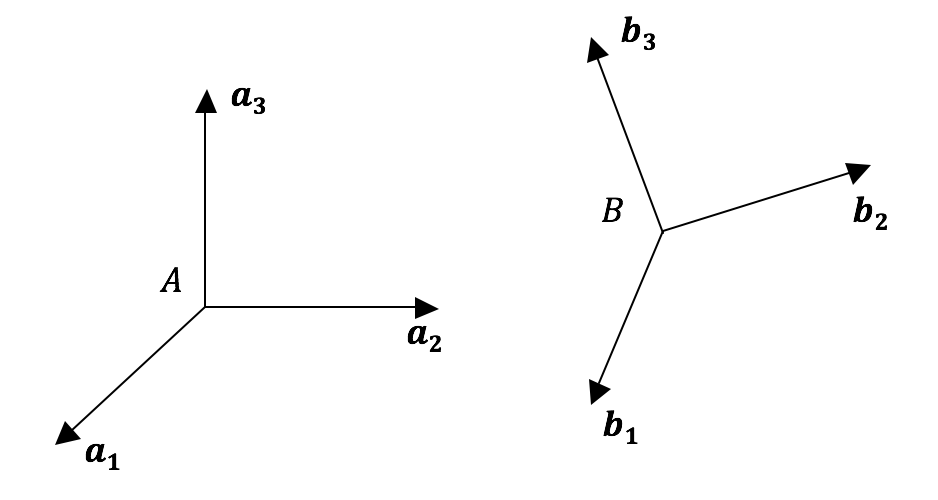
\includegraphics[width=8.3cm]{figures/theTwoFrames}    % The printed column width is 8.4 cm.
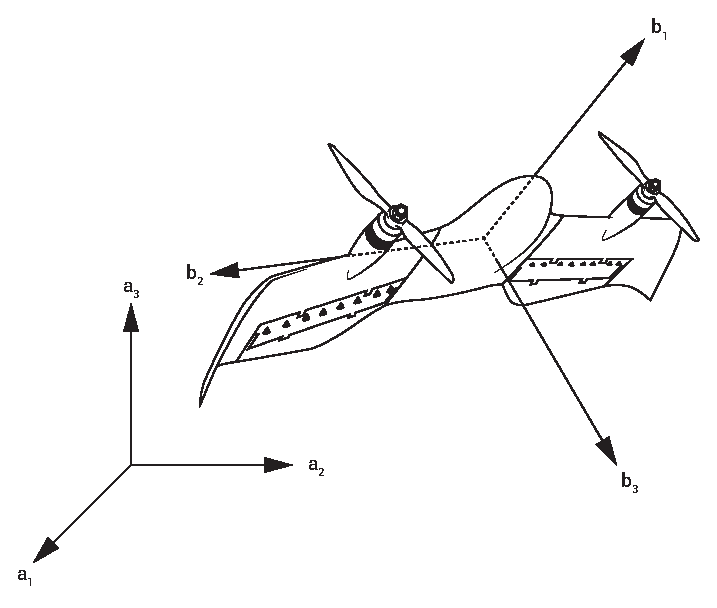
\includegraphics[width=13cm]{figures/DarkoAxesElgiz}    % The printed column width is 8.4 cm.
\caption{Attitude representation is simply specifying the orientation of 
aircraft body axes $b_1, b_2, b_3$ in the reference frame A} 
\label{fig:theTwoFrames}
\end{center}
\end{figure}

Expressing the basis vectors $b_1, b_2, b_3$ of B in terms of basis vectors $a_1, a_2, a_3$ of A such that

\begin{align}
\label{eqn:C_B_A}
\begin{split}
\bm{b_1} = C_{11}\bm{a_1} + C_{12}\bm{a_2} + C_{13}\bm{a_3}  ,
\\
\bm{b_2} = C_{21}\bm{a_1} + C_{22}\bm{a_2} + C_{23}\bm{a_3}  ,
\\
\bm{b_3} = C_{33}\bm{a_1} + C_{32}\bm{a_2} + C_{33}\bm{a_3}  .
\end{split}
\end{align}

where $C_{ij} \equiv {\bm{b_i} \cdot \bm{a_j}} $  is called direction cosine as it corresponds to the cosine of the angle between  $\bm{b_i}$ and $\bm{a_j}$. 
When the previous equation set written in matrix form,

\begin{equation}{\label{eqn:C_B_Amatrix}}
\begin{bmatrix}
\bm{b_1}\\[0.3em]
\bm{b_2}\\[0.3em]
\bm{b_3}\\[0.3em]
\end{bmatrix}
=\,
\begin{bmatrix}
C_{11} & C_{12} & C_{13}\\[0.3em]
C_{11} & C_{12} & C_{13}\\[0.3em]
C_{11} & C_{12} & C_{13}\\[0.3em]
\end{bmatrix}
\,
\begin{bmatrix}
\bm{a_1}\\[0.3em]
\bm{a_2}\\[0.3em]
\bm{a_3}\\[0.3em]
\end{bmatrix}
=\,
\bm{C}^{B/A}
\,
\begin{bmatrix}
\bm{a_1}\\[0.3em]
\bm{a_2}\\[0.3em]
\bm{a_3}\\[0.3em]
\end{bmatrix}
\end{equation} 

Here $\bm{C}^{B/A}$ is called the \emph{direction cosine matrix}, also known as \emph{rotation matrix} or \emph{coordinate transformation matrix} to B from A \cite{wie2008space}.  
The direction cosines, the elements of the direction cosine matrix, are not all independent  \cite{wertz1978spacecraftAttitude}.

The direction cosine matrix is an orthonormal matrix as the basis vectors of each reference frames are orthogonal, so

\begin{equation}
\label{eqn:orthonormality}
\bm{C}^{-1} = \bm{C}^{\rm T}
\end{equation}

and

\begin{equation}
\label{eqn:orthonormality2}
\bm{C}\bm{C}^{\rm T} = \bm{C}^{\rm T}\bm{C} = \mathds{1}
\end{equation}

When the orientation is preserved, an additional condition occurs

\begin{equation}
\label{eqn:noRotation}
\begin{vmatrix}
C\\[0.01em]
\end{vmatrix}
=\,
\mathds{1}
\end{equation}

Matrices satisfying the last two properties belong to special orthogonal group and denoted by SO(3). 
The following relations are valid between $\bm{C}^{B/A}$ - the direction cosine matrix of B relative to A, or the direction cosine matrix to B from A - and $\bm{C}^{A/B}$ - the direction cosine matrix of A relative to B, or the direction cosine matrix to A from B -.

\begin{align}
\label{eqn:C_B_A_vs_C_A_B}
\begin{split}
[\bm{C}^{A/B}]^{-1} = [\bm{C}^{A/B}]^{\rm T} = \bm{C}^{B/A} 
\\
[\bm{C}^{B/A}]^{-1} = [\bm{C}^{B/A}]^{\rm T} = \bm{C}^{A/B}
\end{split}
\end{align}

The direction cosine maps the vectors from reference frame to body frame.  
Let us write an arbitrary vector $\bm{H}$ in the reference frame A and in the body frame B:

\begin{align}
\label{eqn:vectorInRefFrame}
\begin{split}
\bm{H} & = H_1 \bm{a_1} + H_2 \bm{a_2} + H_3 \bm{a_3}
\\
& = H_1^{'} \bm{b_1} + H_2^{'} \bm{b_2} + H_3^{'} \bm{b_3}
\end{split}
\end{align}

Utilization of the direction cosine matrix in the following equation, components of the arbitrary vector $\bm{H}$ is transformed to B from A.

\begin{equation}{\label{transformVectorH}}
\begin{bmatrix}
H_1^{'}\\[0.3em]
H_2^{'}\\[0.3em]
H_3^{'}\\[0.3em]
\end{bmatrix}
=\,
\begin{bmatrix}
 \bm{b_1} \cdot \bm{a_1}  &  \bm{b_1} \cdot \bm{a_2}  &  \bm{b_1} \cdot \bm{a_3} \\[0.3em]
 \bm{b_2} \cdot \bm{a_1}  & \bm{b_2} \cdot \bm{a_2}  & \bm{b_2} \cdot \bm{a_3} \\[0.3em]
 \bm{b_3} \cdot \bm{a_1}  & \bm{b_3} \cdot \bm{a_2}  &  \bm{b_3} \cdot \bm{a_3} \\[0.3em]
\end{bmatrix}
\,
\begin{bmatrix}
 H_1\\[0.3em]
 H_2\\[0.3em]
 H_3\\[0.3em]
\end{bmatrix}
=\,
\bm{C}^{B/A}
\,
\begin{bmatrix}
H_1\\[0.3em]
H_2\\[0.3em]
H_3\\[0.3em]
\end{bmatrix}
\end{equation} 

\subsubsection{Euler Angles}

One of the approaches to represent the attitude is using Euler angles. 
It is a procedure of rotating three times successively about one of the axis of the rotated body fixed reference frame. 
First rotation is about any of the fixed body axes. 
The second rotation is about any of the other two axis which have not been used in the first rotation. 
Third rotation is about one of the axis which have not been used in the second rotation. 
The result is a combination of 12 sets of rotation types. 
A sequence of rotations about three different axes of reference A frame describing the orientation of the body frame B with respect to reference frame A can be represented as

\begin{align}
\label{eqn:sequence}
\begin{split}
{\bm{C}}_3(\theta_{3}) & :      A^{'} \leftarrow A   ,
\\
{\bm{C}}_2(\theta_{2}) & :      A^{''} \leftarrow A^{'}   ,
\\
{\bm{C}}_1(\theta_{1}) & :      A^{'} \leftarrow A^{''}  .
\end{split}
\end{align}

The direction cosine matrix B relative to A can be given as;

\begin{equation}
\label{eqn:sequentialOrientation}
\bm{C}^{B/A}= \bm{C}_{1}(\theta_{1}) \bm{C}_{2}(\theta_{2}) \bm{C}_{3}(\theta_{3})
\end{equation}

where $\theta_{1}$, $\theta_{2}$, $\theta_{3}$ are the Euler angles. $\bm{C}_{i}(\theta_{i})$  
denotes a rotation of angle $\theta_{i}$, about the $i^{th}$ axis of the body frame. The orientation of B with respect to A is given as

\begin{align}{\label{eqn:C_B_AmatrixEuler}}
\begin{split}
\begin{bmatrix}
\bm{b_1}\\[0.3em]
\bm{b_2}\\[0.3em]
\bm{b_3}\\[0.3em]
\end{bmatrix}
& =\,
\bm{C}^{B/A}
\,
\begin{bmatrix}
\bm{a_1}\\[0.3em]
\bm{a_2}\\[0.3em]
\bm{a_3}\\[0.3em]
\end{bmatrix}
\\
& =\,
\begin{bmatrix}
1 & 0 & 0\\[0.3em]
0 & \cos\theta_1 & \sin\theta_1\\[0.3em]
0 & -\sin\theta_1 & \cos\theta_1\\[0.3em]
\end{bmatrix}
\,
\begin{bmatrix}
\cos\theta_2 & 0 & -\sin\theta_2\\[0.3em]
0 & 1 &0\\[0.3em]
\sin\theta_2 & 0 & \cos\theta_2\\[0.3em]
\end{bmatrix}
\,
\begin{bmatrix}
\cos\theta_3 & \sin\theta_3 & 0\\[0.3em]
-\sin\theta_3 & \cos\theta_3 & 0\\[0.3em]
0 & 0 & 1\\[0.3em]
\end{bmatrix}
\\
& =\,
\begin{bmatrix}
\cos\theta_2 \cos\theta_3 & \cos\theta_2 \sin\theta_3 & -\sin\theta_2\\[0.3em]
\sin\theta_1 \sin\theta_2 \cos\theta_3 - \cos\theta_1 \sin\theta_3 & \sin\theta_1 \sin\theta_2 \cos\theta_3 + \cos\theta_1 \cos\theta_1 \cos\theta_3 & \sin\theta_1 \cos\theta_2\\[0.3em]
\cos\theta_1 \sin\theta_2 \cos\theta_3 + \sin\theta_1 \sin\theta_3 & \cos\theta_1 \sin\theta_2 \sin\theta_3 - \sin\theta_1 \cos\theta_3 & \cos\theta_1 \cos\theta_2\\[0.3em]
\end{bmatrix}
\end{split}
\end{align}

If the set of rotations is selected in a different way, such as 

\begin{align}
\label{eqn:sequence2}
\begin{split}
{\bm{C}}_2(\theta_{2}) & :      A^{'} \leftarrow A   ,
\\
{\bm{C}}_3(\theta_{3}) & :      A^{''} \leftarrow A^{'}   ,
\\
{\bm{C}}_1(\theta_{1}) & :      A^{'} \leftarrow A^{''}  .
\end{split}
\end{align}

then the direction cosine matrix would differ from the previous one.

\subsubsection{Quaternions}

The idea behind this representation is the Euler's \emph{eigen-axis rotation} theorem. 
According to Euler, \say{the most general displacement of a rigid body with one point fixed is a rotation about some axis.} In other words, it states that there exists a unit vector $\bm{e}$, with the property

\begin{equation}
\label{eqn:quat1}
\bm{C}\bm{e}= \bm{e}
\end{equation}

$\bm{e}$ vector has the same components in body and reference frames such that

\begin{align}
\label{eqn:quat2}
\begin{split}
\bm{e} & = e_1 \bm{a_1} + e_2 \bm{a_2} + e_3 \bm{a_3}
\\
& = e_1 \bm{b_1} + e_2 \bm{b_2} + e_3 \bm{b_3}
\end{split}
\end{align}
 
Rotating a rigid body about this axis $\bm{e}$, rotation from any given orientation to any other orientation can be achieved. 
Such a rotation is named after the Swiss mathematician and theoretical physicist Leonard Euler (1707-1783), \emph{Euler axis}.

\emph{Euler symmetric parameters}, also known as \emph{quaternions}, are defined as:
 
 \begin{equation}
 \label{eqn:quat3}
\bm{q}
=\,
\begin{bmatrix}
q_0\\[0.3em]
q_1\\[0.3em]
q_2\\[0.3em]
q_3\\[0.3em]
\end{bmatrix}
=\,
\begin{bmatrix}
\cos(\phi/2)\\[0.3em]
e_1 \sin(\phi/2)\\[0.3em]
e_2 \sin(\phi/2)\\[0.3em]
e_3 \sin(\phi/2)\\[0.3em]
\end{bmatrix}
\end{equation}
 
Where $\phi$ is the \emph{Euler rotation angle}. 
Hamilton (1805-1865) is considered to be the first one to mention quaternions. 
For ease of the mathematical representations, we define a vector such as

\begin{equation}
\label{eqn:quat3}
\bm{q} = \bm{e}\sin{\phi/2}
\end{equation}

Euler symmetric parameters are not independent, and satisfy the constraint

\begin{equation}
\label{eqn:quatNormConstraint}
\bm{q}^{\rm T} \bm{q} + q_0^2 = q_0^2 + q_1^2 +q_1^2 +q_3^2 = 1
\end{equation}

The direction cosine matrix can also be written in terms of quaternions as below

\begin{align}\label{eqn:Cquat}
\begin{split}
C(\bm{q})
 & =\,
\begin{bmatrix}
q_0^2 + q_1^2 - q_2^2 - q_3^2 & 2(q_1 q_2 + q_3 q_0) & 2(q_1 q_3 - q_2 q_0)\\[0.3em]
2(q_1 q_2 - q_3 q_0) & q_0^2 - q_1^2 + q_2^2 - q_3^2 & 2(q_2 q_3 + q_1 q_0)\\[0.3em]
2(q_1 q_3 + q_2 q_0) & 2(q_2 q_3 - q_1 q_0) & -q_1^2 - q_2^2 + q_3^2 + q_0^2\\[0.3em]
\end{bmatrix}
\\
& = (q_0^2 - \bm{q}^{\rm T}\bm{q} )\mathds{1} + 2\bm{q}\bm{q}^{\rm T} - 2q_0\bm{Q}
\end{split}
\end{align}
 
where

\begin{equation}
\label{eqn:Qmatrix}
\bm{Q}
=\,
\begin{bmatrix}
0 & - q_3 & q_2 \\[0.3em]
q_3 & 0 & - q_1 \\[0.3em]
- q_2 & q_1 & 0\\[0.3em]
\end{bmatrix}
\end{equation}

Given the direction cosine matrix, quaternions can be calculated as

\begin{align}\label{eqn:quat4}
\begin{split}
\bm{q}
& =\,
\begin{bmatrix}
q_1\\[0.3em]
q_2\\[0.3em]
q_3\\[0.3em]
\end{bmatrix}
 =\,
\frac{1}{4q_0}
\begin{bmatrix}
C_{23} - C_{32}\\[0.3em]
C_{31} - C_{13}\\[0.3em]
C_{12} - C_{21}\\[0.3em]
\end{bmatrix}
\\
q_0
& =\,
\pm{\frac{1}{2}}{(1 + C_{11} + C_{22} + C_{33})}^{\frac{1}{2}}
\end{split}
\end{align}

\subsubsection{Attitude parametrization selection}

In 1776, Euler showed that SO(3) has three dimensions \cite{stuelpnagel1964parametrization}. 
Representations with more than three parameters are subject to constraints. 
Also, \cite{stuelpnagel1964parametrization} states that no parameter set 
can be both global and nonsingular. 
So, we are faced with choosing the representation parameters either singular or redundant. 
Euler angle representation has its advantages like having a clear physical interpretation and minimum parameter set achieving no redundancy. 
But due to their important disadvantage, the possibility of having singularities when describing motion, Euler angles are not selected to represent attitude in this study.
The Gibbs vector is not very often used, and can be thought that it is an interval step on the way of quaternion parametrization. 
There are other representation types, which are not very often 
preferred, such as the axis-azimuth representation, which will not be mentioned  in this thesis. 
Quaternion (Euler symmetric parameters) representation takes the lead for this study due to their advantageous in simulations, and having no singularities.
Another advantage of quaternions is that, the kinematic equations are linear in terms of quaternions. 
Also, quaternion multiplication offers a useful way of expressing composite rotations. 
With all these preferable properties, quaternions are the choice for attitude representations for many attitude control missions. ~\ref{tab:attRepSelection} shows a brief comparison of attitude representations \cite{bak1999spacecraft}.\\
In the previous sections, a variety of parameters to represent rotations are identified and inherent properties of each technique have been examined. 
Now it is time to find out how to represent attitude depending on time, namely the equations of motion. 
Equations of motion is generally presented in two sections: the kinematic equations and dynamic equations. 
The kinematic equations provide the relations between the time derivative of the attitude representation and the angular velocity, while the dynamics (or kinetics) describe the development of angular velocities under influence of external moments.


\label{tab:attRepSelection}
\begin{center}
 \begin{tabular}{||c || c | c ||}
 \hline
 &Number of  &  \\ [0.5ex] 
Representation &parameter set & Properties \\ [0.5ex] 
 \hline\hline
& & Minimal set\\ 
& & Clear physical interpretation\\ 
& & Often computed directly\\ 
 Euler angles   & 3 & Trigonometric functions in rotation matrix \\ 
& & No simple composition rule \\ 
& & Singular for certain rotations \\ 
& & Trigonometric functions in kinematic relation \\ 
 \hline
& & Easy orthogonality of rotation matrix\\ 
& & Bilinear composition rule\\ 
& & Not singular at any rotation\\ 
Quaternions   & 4 & Linear kinematic equations \\ 
& & No clear physical interpretation \\ 
& &One redundant parameter \\ 
& & Simple kinematic relation \\ 
 \hline
& & Minimal set\\ 
Gibbs vector   & 4 & Clear composition rule\\ 
& & Singular for certain rotations \\ 
& & Simple kinematic relation \\[1ex] 
 \hline
\end{tabular}
\end{center}

%\begin{table}
%\caption{Armadillos}
%\label{arm:table}
%\begin{center}
%\begin{tabular}{||l|l||}\hline
%Armadillos & are \\\hline
%our	   & friends \\\hline
%\end{tabular}
%\end{center}
%\end{table}


\subsection{Attitude kinematics}

The time evolution of attitude is identified by a set of first order differential equations called the kinematic equations. 
The angular velocity of a reference frame B with respect a reference frame A, given in the B frame can be written as follows

\begin{equation}\label{eqn:quaternion1}
\bm{\omega}
 =\,
\omega_1 \bm{b_1} + \omega_2 \bm{b_2} + \omega_3 \bm{b_3}
\end{equation}

Recalling Eq. ~\ref{eqn:C_B_Amatrix} and orthonomality property in Eq. ~\ref{eqn:orthonormality}

\begin{equation}{\label{eqn:kinematicsDerivation1}}
\begin{bmatrix}
\bm{a_1}\\[0.2em]
\bm{a_2}\\[0.2em]
\bm{a_3}\\[0.2em]
\end{bmatrix}
=\,
\Big[{\bm{C}_B^{B/A}}\Big]^{-1}
\,
\begin{bmatrix}
\bm{b_1}\\[0.2em]
\bm{b_2}\\[0.2em]
\bm{b_3}\\[0.2em]
\end{bmatrix}
=\,
\Big[{\bm{C}_B^{B/A}}\Big]^{\rm T}
\,
\begin{bmatrix}
\bm{b_1}\\[0.2em]
\bm{b_2}\\[0.2em]
\bm{b_3}\\[0.2em]
\end{bmatrix}
\end{equation} 

Taking the time derivative with respect to frame A

\begin{align}{\label{eqn:C_B_Amatrix_timeDerivative}}
\begin{split}
\frac{d}{dt}
\left.
\begin{bmatrix}
\bm{a_1}\\[0.2em]
\bm{a_2}\\[0.2em]
\bm{a_3}\\[0.2em]
\end{bmatrix}
\right|_A &=\,
\Big[{\dot{\bm{C}}_B^{B/A}}\Big]^{\rm T}
\,
\begin{bmatrix}
\bm{b_1}\\[0.2em]
\bm{b_2}\\[0.2em]
\bm{b_3}\\[0.2em]
\end{bmatrix}
+\,
\Big[{\bm{C}_B^{B/A}}\Big]^{\rm T}
\,
\begin{bmatrix}
\dot{\bm{b_1}}\\[0.2em]
\dot{\bm{b_2}}\\[0.2em]
\dot{\bm{b_3}}\\[0.2em]
\end{bmatrix}
=\,
\Big[{\dot{\bm{C}}_B^{B/A}}\Big]^{\rm T}
\,
\begin{bmatrix}
\bm{b_1}\\[0.2em]
\bm{b_2}\\[0.2em]
\bm{b_3}\\[0.2em]
\end{bmatrix}
+\,
\Big[{\bm{C}_B^{B/A}}\Big]^{\rm T}
\,
\begin{bmatrix}
\bm{\omega} \times \bm{b_1}\\[0.2em]
\bm{\omega} \times \bm{b_2}\\[0.2em]
\bm{\omega} \times \bm{b_3}\\[0.2em]
\end{bmatrix}
\\
& =\,
\Big[{\dot{\bm{C}}_B^{B/A}}\Big]^{\rm T}
\,
\begin{bmatrix}
\bm{b_1}\\[0.2em]
\bm{b_2}\\[0.2em]
\bm{b_3}\\[0.2em]
\end{bmatrix}
+\,
\Big[{\bm{C}_B^{B/A}}\Big]^{\rm T}
\,
\begin{bmatrix}
0 & - \omega_3 & \omega_2 \\[0.3em]
\omega_3 & 0 & - \omega_1 \\[0.3em]
- \omega_2 & \omega_1 & 0\\[0.3em]
\end{bmatrix}
\,
\begin{bmatrix}
\bm{b_1}\\[0.2em]
\bm{b_2}\\[0.2em]
\bm{b_3}\\[0.2em]
\end{bmatrix}
\end{split}
\end{align}

If the skew-symmetric matrix can be represented as $\bm{\Omega}$

\begin{equation}\label{eqn:Qmatrix}
\bm{\Omega}
=\,
\begin{bmatrix}
0 & - \omega_3 & \omega_2 \\[0.3em]
\omega_3 & 0 & - \omega_1 \\[0.3em]
- \omega_2 & \omega_1 & 0\\[0.3em]
\end{bmatrix}
\end{equation}

and rearrange the terms

\begin{equation}{\label{eqn:C_dot_T_C_T_Omega}}
\bigg[\Big[{\dot{\bm{C}}_B^{B/A}}\Big]^{\rm T} - \Big[{\bm{C}_B^{B/A}}\Big]^{\rm T} \bm{\Omega} \bigg]
\,
\begin{bmatrix}
\bm{b_1}\\[0.2em]
\bm{b_2}\\[0.2em]
\bm{b_3}\\[0.2em]
\end{bmatrix}
 =\,
\begin{bmatrix}
0\\[0.2em]
0\\[0.2em]
0\\[0.2em]
\end{bmatrix}
\end{equation}

implies

\begin{equation}{\label{eqn:C_dot_T_C_T_Omega2}}
\bigg[\Big[{\dot{\bm{C}}_B^{B/A}}\Big]^{\rm T} - \Big[{\bm{C}_B^{B/A}}\Big]^{\rm T} \bm{\Omega} \bigg]
 =\,
\bm{0}
\end{equation}

Taking the transpose and using the relationship $\Omega^{\rm T} = - \Omega$, the kinematic differential equation for the direction cosine matrix can be written as,

\begin{equation}{\label{eqn:kinematicEquDQM}}
{\dot{\bm{C}}_B^{B/A}} + \bm{\Omega} {\bm{C}_B^{B/A}}
 =\,
\bm{0}
\end{equation}

Angular velocity components, given in the B reference frame can be written as

\begin{align}{\label{eqn:angVelocityKinematics}}
\begin{split}
\omega_1 & = \dot{C}_{21} C_{31} + \dot{C}_{22} C_{32} + \dot{C}_{23} C_{33} \\
\omega_2 & = \dot{C}_{31} C_{11} + \dot{C}_{32} C_{12} + \dot{C}_{33} C_{13} \\
\omega_3 & = \dot{C}_{11} C_{21} + \dot{C}_{12} C_{22} + \dot{C}_{13} C_{23} \\
\end{split}
\end{align}

From that point, derivation depends on the attitude parameters used. 
When the direction cosines and their derivatives are substituted with their equals in terms of Euler angles, the result will give the time dependence of Euler angles. 
But in this study, due to the reasons discussed before, quaternions are selected to represent the attitude, so the direction cosines will be written in terms of quaternions,

\begin{align}{\label{eqn:angVelocityQuaternion}}
\begin{split}
\omega_1 & = 2 (\dot{q}_1 q_0 + \dot{q}_2 q_3 - \dot{q}_3 q_2 - \dot{q}_0 q_1) \\
\omega_2 & = 2 (\dot{q}_2 q_0 + \dot{q}_3 q_1 - \dot{q}_1 q_3 - \dot{q}_0 q_2) \\
\omega_3 & = 2 (\dot{q}_3 q_0 + \dot{q}_1 q_2 - \dot{q}_2 q_1 - \dot{q}_2 q_3)\\
\end{split}
\end{align}

Fourth equation comes from the differentiation of the quaternion norm constraint;

\begin{equation}{\label{eqn:kinematicEquDQM}}
0 = 2 (- \dot{q}_0 q_0 + \dot{q}_1 q_1 + \dot{q}_2 q_2 - \dot{q}_3 q_3)
\end{equation}

Writing in matrix form;

\begin{equation}{\label{eqn:kinematicEquAngVel}}
\begin{bmatrix}
0\\[0.2em]
\omega_1\\[0.2em]
\omega_2\\[0.2em]
\omega_3\\[0.2em]
\end{bmatrix}
 =\,
 2\,
\begin{bmatrix}
q_1 & q_2 & q_3 & q_0 \\[0.2em]
q_0 & q_3 & -q_2 & -q_1 \\[0.2em]
-q_3 & q_0 & q_1 & -q_2 \\[0.2em]
q_2 & -q_1 & q_0 & -q_3 \\[0.2em]
\end{bmatrix}
\,
\begin{bmatrix}
\dot{q}_0\\[0.2em]
\dot{q}_1\\[0.2em]
\dot{q}_2\\[0.2em]
\dot{q}_3\\[0.2em]
\end{bmatrix}
\end{equation}
 
As the matrix which is composed of quaternions is an orthonormal matrix, the kinematic equations of motion in terms of quaternions can be given as \cite{wie2008space}

\begin{align} \label{eqn:kinematicArrange}
\begin{split}
\begin{bmatrix}
\dot{q}_0\\[0.2em]
\dot{q}_1\\[0.2em]
\dot{q}_2\\[0.2em]
\dot{q}_3\\[0.2em]
\end{bmatrix}
& =\,
\frac{1}{2}
\,
\begin{bmatrix}
-q_1 & -q_2 & -q_3 & q_0 \\[0.2em]
q_4 & -q_3 & q_2 & q_1 \\[0.2em]
q_3 & q_4 & -q_1 & q_2 \\[0.2em]
-q_2 & -q_1 & q_4 & q_3 \\[0.2em]
\end{bmatrix}
\,
\begin{bmatrix}
0\\[0.2em]
\omega_1\\[0.2em]
\omega_2\\[0.2em]
\omega_3\\[0.2em]
\end{bmatrix} \\
& =\,
\frac{1}{2}
\,
\begin{bmatrix}
-\omega_1 & -\omega_2 & -\omega_3 & 0 \\[0.2em]
0 & \omega_3 & -\omega_2 & \omega_1 \\[0.2em]
-\omega_3 & 0 & \omega_1 & \omega_2 \\[0.2em]
\omega_2 & -\omega_1 & 0 & \omega_3 \\[0.2em]
\end{bmatrix}
\begin{bmatrix}
q_0\\[0.2em]
q_1\\[0.2em]
q_2\\[0.2em]
q_3\\[0.2em]
\end{bmatrix}
\end{split}
\end{align}

And in a more compact form;

\begin{align}{\label{eqn:compactKinematics}}
\begin{split}
\dot{q}_0 &= -\frac{1}{2} \bm{q}_\nu^T \bm{\omega}_{b/n}^b\\
\dot{\bm{q}}_\nu &= \frac{1}{2}\Big(\bm{q}_\nu^\times + q_0 \bm{I}_3 \Big) \bm{\omega}_{b/n}^b \\
\end{split}
\end{align}

where

\begin{equation}
\bm{x} ^ \times= \begin{bmatrix} 
0 & -x_3 & x_2 \\
x_3 & 0 & -x_1 \\
-x_2 & x_1 & 0 \\
 \end{bmatrix}
\end{equation}

\subsection{Attitude dynamics}

The equation describing the rotational motion of a rigid body moving relative to an inertial frame can written as \cite{wie2008space}

\begin{equation}{\label{eqn:kinematicEquDQM}}
\int \bm{r} \times \ddot{\bm{R}} dm = \bm{M_0}
\end{equation}

Here the rotation of the rigid body takes place about an arbitrary point O. 
Let us take an infinitesimal mass element $dm$. 
In Fig.\ref{fig:attDyn1}, $\bm{r}$ is the position vector of $dm$ relative to O, $\bm{R}$ is the position vector of $dm$ relative to the origin of the inertial frame, $\ddot{\bm{R}}$ is the acceleration of $dm$, $\bm{M_0}$ is the total external torque about point O.

\begin{figure}
\begin{center}
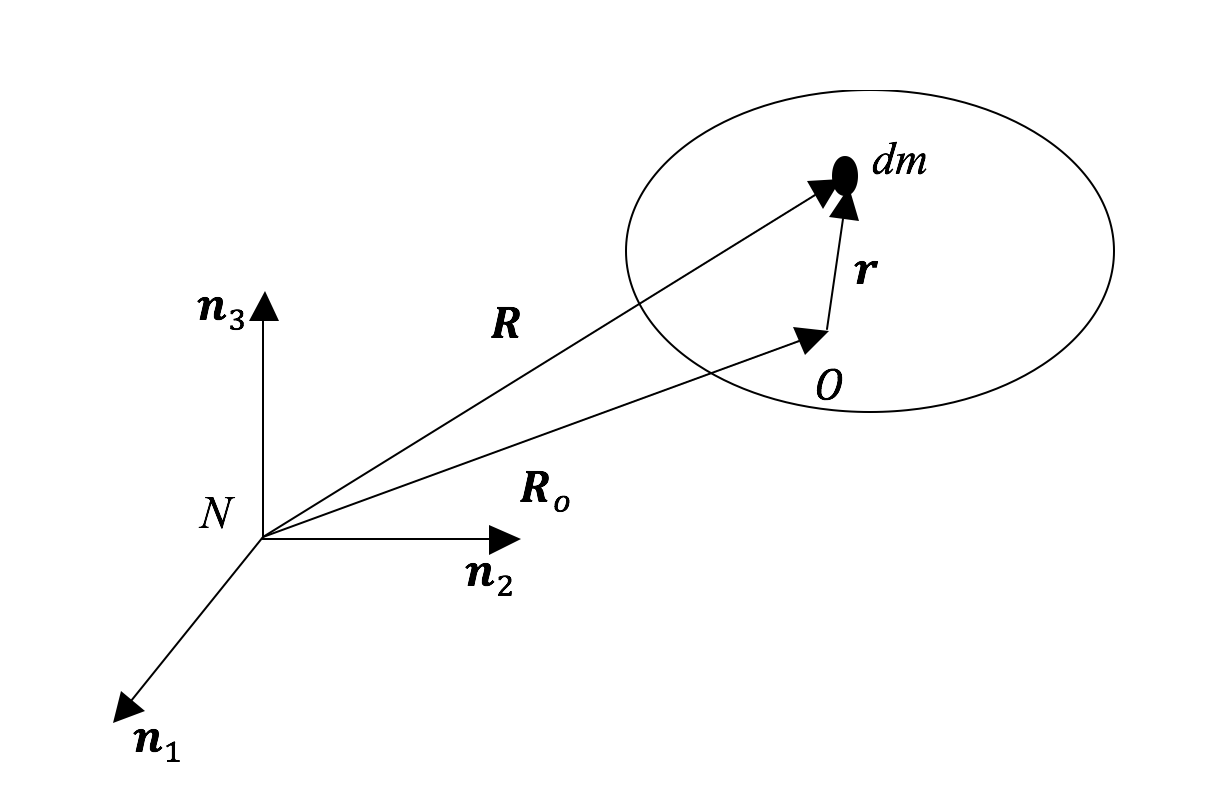
\includegraphics[width=9cm]{figures/attDyn1}    % The printed column width is 8.4 cm.
\caption{Rigid body rotating about an arbitrary point O, given in the N frame} 
\label{fig:attDyn1}
\end{center}
\end{figure}

\begin{figure}
\begin{center}
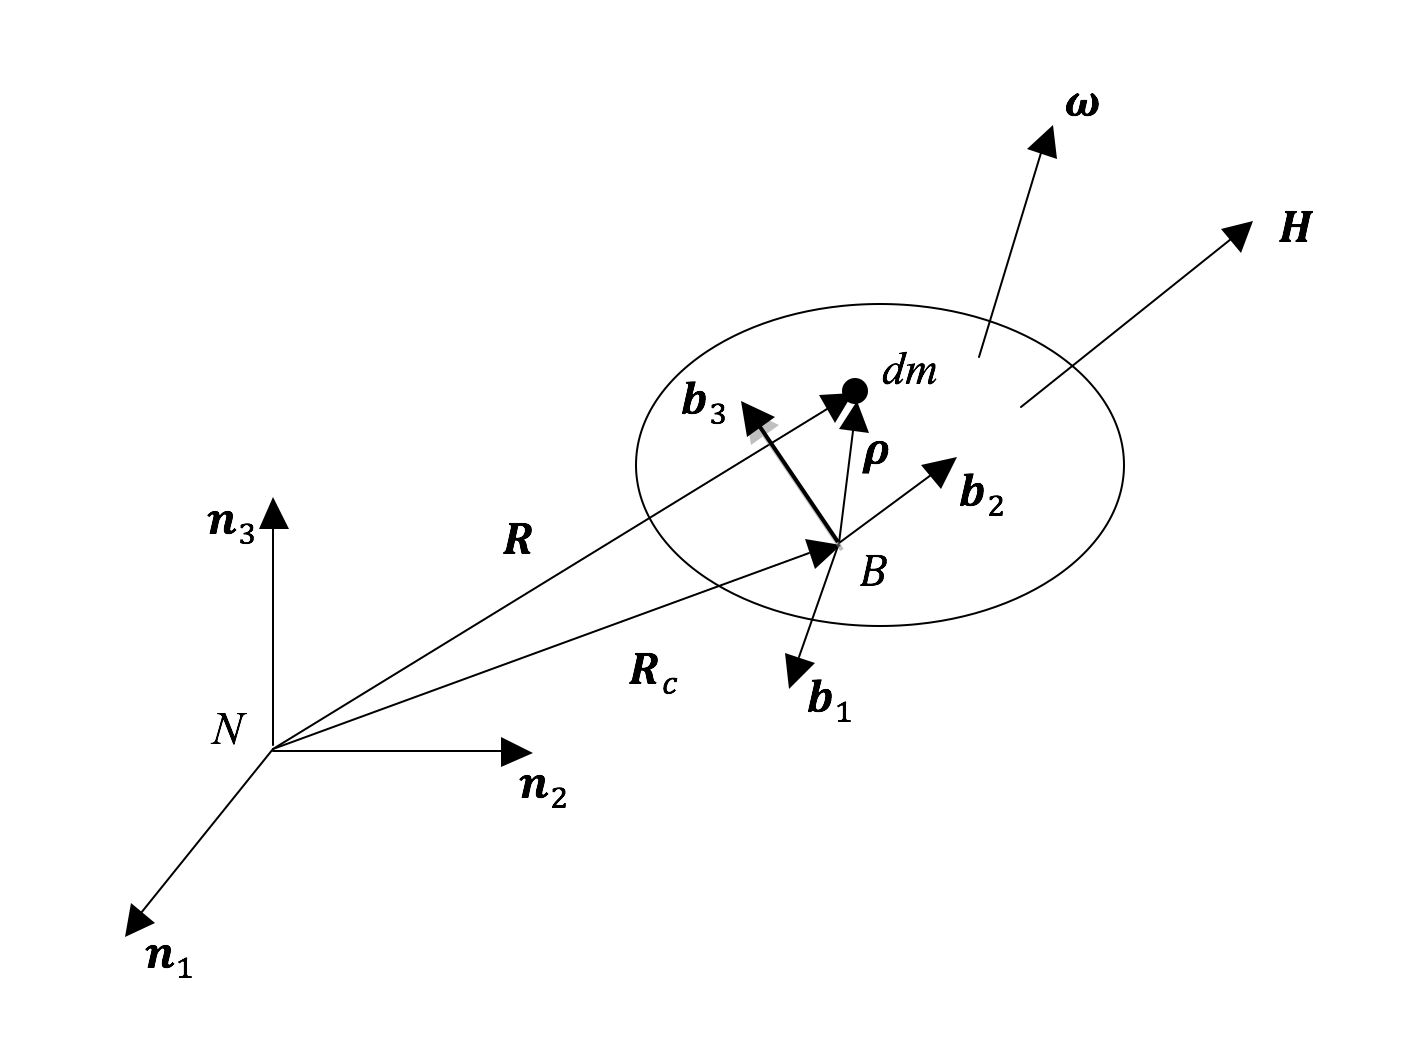
\includegraphics[width=10cm]{figures/attDyn2}    % The printed column width is 8.4 cm.
\caption{Rigid body rotating about an arbitrary point O, given in the N frame} 
\label{fig:attDyn2}
\end{center}
\end{figure}

Now, let us take a body fixed frame B originated at the center of mass of the rigid body as shown in Fig. \ref{fig:attDyn2}. 
In Fig. \ref{fig:attDyn2}, $\bm{\rho}$  is the position vector of $dm$ mass with respect to center of mass of the rigid body, $\bm{R}_c$ is the position vector of the center of mass of the rigid body with respect to the origin of the inertial frame N, and $\bm{R}$ is the position vector of dm with respect to the origin of the inertial frame N. 

The angular velocity of the rigid body in the inertial frame N is denoted as $\bm{\omega} \equiv \bm{\omega}_B^{B/N}$. 
It represents the angular velocity of the body frame B with respect to inertial frame N given in the body frame B. 
Angular momentum vector $\bm{H}$ a rigid body about its center of mass given as,

\begin{equation}{\label{eqn:kinematicEquDQM}}
\bm{H} = \int \bm{\rho} \times \dot{\bm{R}} dm
\end{equation}

Since $\bm{R}_C$ is constant

\begin{equation}{\label{eqn:kinematicEquDQM}}
\dot{\bm{R}} = \dot{\bm{R}}_C + \dot{\bm{\rho}} = \dot{\bm{\rho}}
\end{equation}

And from rigidity of the body,

\begin{equation}{\label{eqn:kinematicEquDQM}}
\dot{\bm{\rho}} \equiv \bigg\{ \frac{d\bm{\rho}}{dt} \bigg\}_N = \bigg\{ \frac{d\bm{\rho}}{dt} \bigg\}_B + \bm{\omega} \times \bm{\rho} = \bm{\omega} \times \bm{\rho}
\end{equation}

Then the angular momentum is given as;

\begin{equation}{\label{eqn:kinematicEquDQM}}
\bm{H} = \int \bm{\rho} \times \dot{\bm{R}} dm = \int \bm{\rho} \times \dot{\bm{\rho}} dm = \int \bm{\rho} \times  (\bm{\omega} \times \bm{\rho} )dm
\end{equation}

The components of $\bm{\rho}$ and $\bm{\omega}$ in the body frame B is written as;

\begin{align}{\label{eqn:omega_and_rho}}
\begin{split}
\bm{\rho} & = \rho_1 \bm{b}_1 + \rho_2 \bm{b}_2 + \rho_3 \bm{b}_3 \\
\bm{\omega} & = \omega_1 \bm{b}_1 + \omega_2 \bm{b}_2 + \omega_3 \bm{b}_3 \\
\end{split}
\end{align}

Then the angular momentum can be written as;

\begin{equation}{\label{eqn:angMomentumComp}}
\bm{H} = H_1 \bm{b}_1 + H_2 \bm{b}_2 + H_3 \bm{b}_3 
\end{equation}

where

\begin{align}{\label{eqn:angularMomentum1}}
\begin{split}
H_1 & = I_{11} \omega_1 + I_{12} \omega_2 + I_{13} \omega_3 \\
H_2 & = I_{21} \omega_1 + I_{22} \omega_2 + I_{23} \omega_3 \\
H_3 & = I_{31} \omega_1 + I_{32} \omega_2 + I_{33} \omega_3 \\
\end{split}
\end{align}

Writing in matrix form gives,

\begin{equation}{\label{eqn:angularMomentumInMatrixForm}}
\begin{bmatrix}
H_1\\[0.2em]
H_2\\[0.2em]
H_3\\[0.2em]
\end{bmatrix}
 =\,
\begin{bmatrix}
I_{11} & I_{12} & I_{13} \\[0.2em]
I_{21} & I_{22} & I_{23} \\[0.2em]
I_{31} & I_{32} &I_{33} \\[0.2em]
\end{bmatrix}
\,
\begin{bmatrix}
\omega_1\\[0.2em]
\omega_2\\[0.2em]
\omega_3\\[0.2em]
\end{bmatrix}
\end{equation}

and in compact form

\begin{equation}{\label{eqn:angMomentumComp2}}
\bm{H} = \bm{I} \bm{\omega}
\end{equation}

where $\bm{I}$  is called the inertia matrix of the rigid body about a body fixed reference frame B originating at the center of mass of the rigid body.

Let us write a set of axes to achieve all the products of inertia, or all the elements of the inertia matrix other than diagonal elements, are zero. 
This set is called the principal axes and the moments of inertia are called the principal moments of inertia. 
Assuming the axes of the body reference frame B are the principal axes, then the equation for the angular momentum becomes;

\begin{equation}{\label{eqn:angularMomentumInPrincipleAxes}}
\begin{bmatrix}
H_1\\[0.2em]
H_2\\[0.2em]
H_3\\[0.2em]
\end{bmatrix}
 =\,
\begin{bmatrix}
I_{11} & 0 & 0 \\[0.2em]
0 & I_{22} & 0 \\[0.2em]
0 & 0 &I_{33} \\[0.2em]
\end{bmatrix}
\,
\begin{bmatrix}
\omega_1\\[0.2em]
\omega_2\\[0.2em]
\omega_3\\[0.2em]
\end{bmatrix}
\end{equation}

Now, it is time to express the rotational equations of motion - also  known as Euler's equations of motion - for a rigid body.  Remember the angular momentum equation

\begin{equation}{\label{eqn:angMomentumComp}}
\bm{M} = \dot{\bm{H}} 
\end{equation}

where $\bm{H}$ is the angular momentum vector of the rigid body about its center of mass and  $\bm{M}$ is the external moment acting on the rigid body about its center of mass.  We can also write it as;

\begin{equation}{\label{eqn:attDynDerivation1}}
\dot{\bm{H}} = \bigg\{ \frac{d\bm{H}}{dt} \bigg\}_N 
=\,
\bigg\{ \frac{d\bm{H}}{dt} \bigg\}_B  + \bm{\omega}_B^{B/N} \times \bm{H}
 =\,
  \bm{M}
\end{equation}

By taking the time derivative of Eq. \ref{eqn:angMomentumComp2}, assuming the inertia is not dependent on time, and evaluating in  Eq. \ref{eqn:attDynDerivation1}, Euler's rotational equation of motion can be written as 

\begin{equation}{\label{eqn:kinematicEquDQM}}
\dot{\bm{\omega}}_B^{B/N}  = \bm{I}_B^{-1} (\bm{M}_B - \bm{\omega}_B^{B/N} \times \bm{I}_B \bm{\omega}_B^{B/N}) 
\end{equation}

\section{Translation modeling}

The movement of any object can be represented by changes in its location (translation) or changes in its attitude (rotation) or a combination of both. 
Studying aircraft motion is complicated since those two motions are coupled, e.g a rotation might cause a change in aerodynamic forces which affects the translation. 
Thus, to ease the modeling process, the aircraft is assumed to be a point mass, all its mass collected at its center of gravity, while it translates from one point to the other.
Then the motion of the that point, at its center of gravity, is described by Newton's laws of motion.
The translations are in direct response to external forces, namely the lift, drag, thrust and weight.
Unfortunately those forces depend on the attitude of the aircraft.

\subsection{Translational kinematics}

Time change of the position of the aircraft $\bm{x}_n$ expressed in the navigation frame can be written in terms of translational velocity $\bm{v}_b$ expressed in the body frame as

\begin{align}{\label{eqn:translationalKinematics1}}
\begin{split}
\dot{\bm{x}}_n & = \frac{d}{dt} \big( \bm{x}_n \big) \\
                        & = \frac{d}{dt} \big(\bm{C}_b^n \bm{x}_b \big) \\
                        & = \dot{\bm{C}}_b^n \bm{x}_b + \bm{C}_b^n  \dot{\bm{x}}_b \\
                        & = \bm{C}_b^n \bm{v}_b
\end{split}
\end{align}

using $\bm{x}_b=0$. Eq. \ref{eqn:translationalKinematics1} can also be represented in matrix form pointing the elements of the vectors as

\begin{equation}{\label{eqn:angularMomentumInPrincipleAxes}}
\begin{bmatrix}
\dot{x}_N\\[0.2em]
\dot{x}_E\\[0.2em]
\dot{x}_D\\[0.2em]
\end{bmatrix}
 =\,
\bm{C}_b^n
\,
\begin{bmatrix}
u\\[0.2em]
v\\[0.2em]
w\\[0.2em]
\end{bmatrix}
\end{equation}

\subsection{Translational dynamics}

The aircraft is assumed to be a point mass, all its mass collected at its center of gravity, while it translates from one point to the other.
Then the motion of the that point, at its center of gravity, is described by Newton's laws of motion.
The translations are in direct response to external forces, namely the lift, drag, thrust and weight.
From now on, the aircraft will be assumed to be flying over a small region compared to size of the Earth so that the Earth is locally flat (good old times) to neglect centripetal acceleration (due to Earth's curvature). 
Another assumption is that the frame attached to Earth being an inertial frame by ignoring Coriolis acceleration so that Newton's laws apply. 

\begin{equation}{\label{eqn:newtonsSecondLaw}}
\sum_j \bm{F}_j = \left. \frac{d}{dt} \big( m \bm{v} \big) \right|_A 
\end{equation}

Unfortunately those forces that directly effect the translation depend on the attitude of the aircraft, complicating the dynamics.

\subsubsection{Model of aerodynamic forces}




\section{Drone model}


In this section parameters for two different drone is given, ETH model aircraft and MAKO model. 

As an addition to the aerodynamic coefficients and stability derivatives, it is useful to have the moments of inertia of the aircraft so that one can use the model in a simulator. 
For that purpose, the aircraft is hanged by two strings, at different orientations, as shown in Figure \ref{fig:inertia}, and measurements performed by timing the oscillation period for each axis. 
The resultant moment of inertias are given Table ~\ref{arm:MAKO}. 

\begin{figure}
\centering
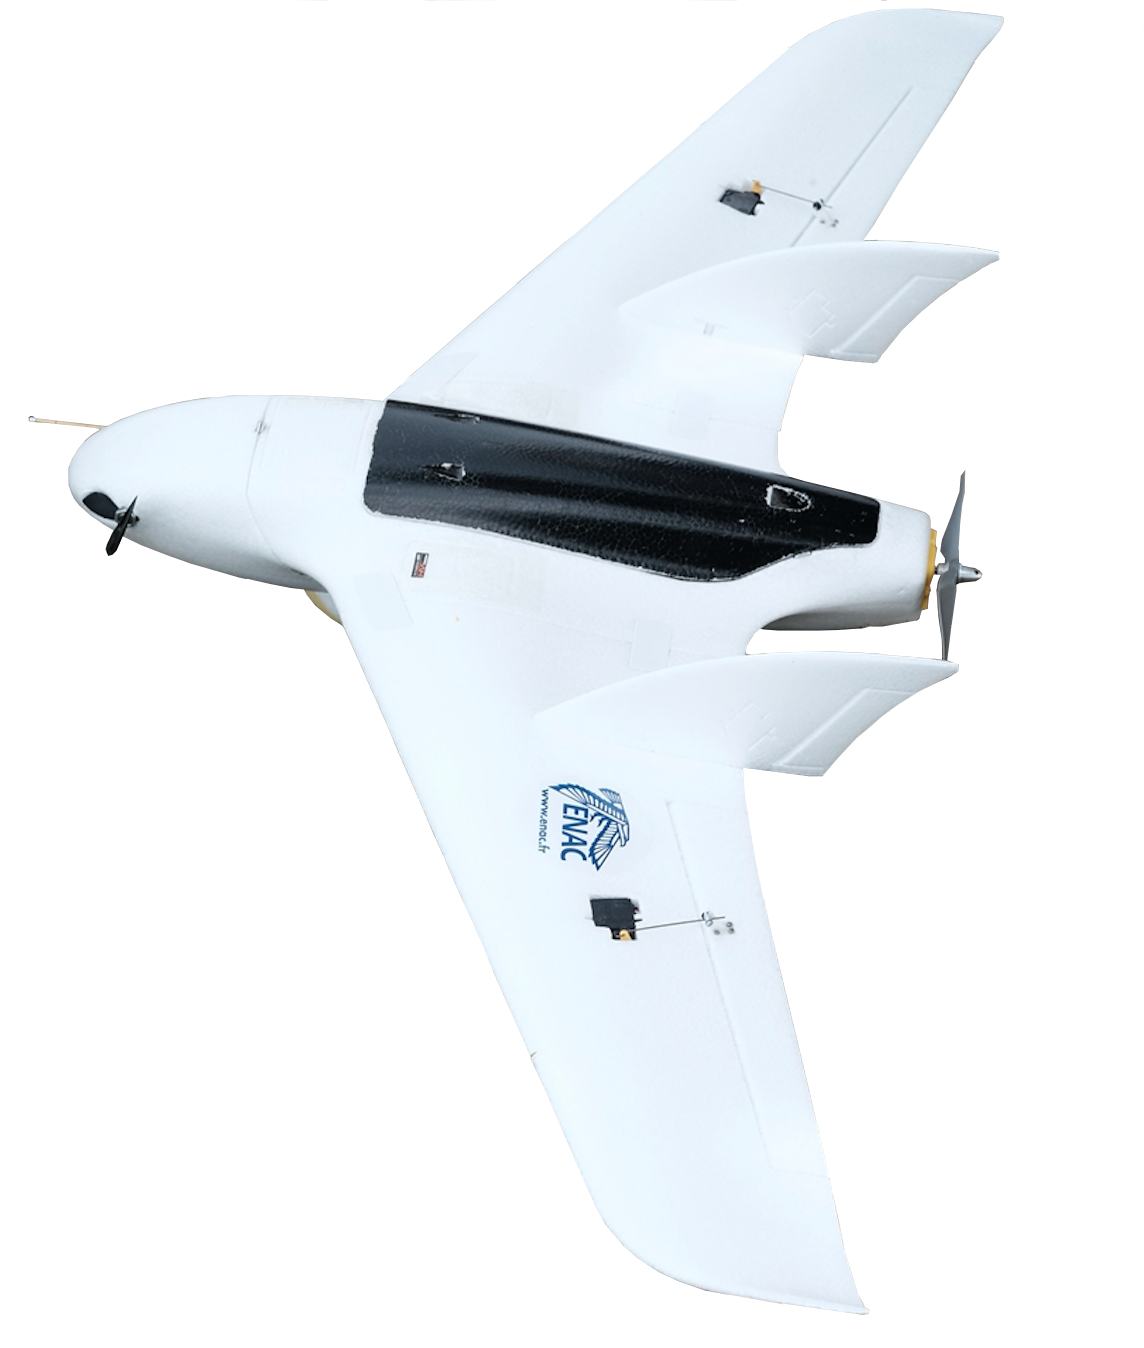
\includegraphics[width=0.7\columnwidth]{figures/makoEmptyBack}
\caption{MAKO}
\label{figure:mako}
\end{figure}


 \begin{figure*}[!ht]
      \centering
      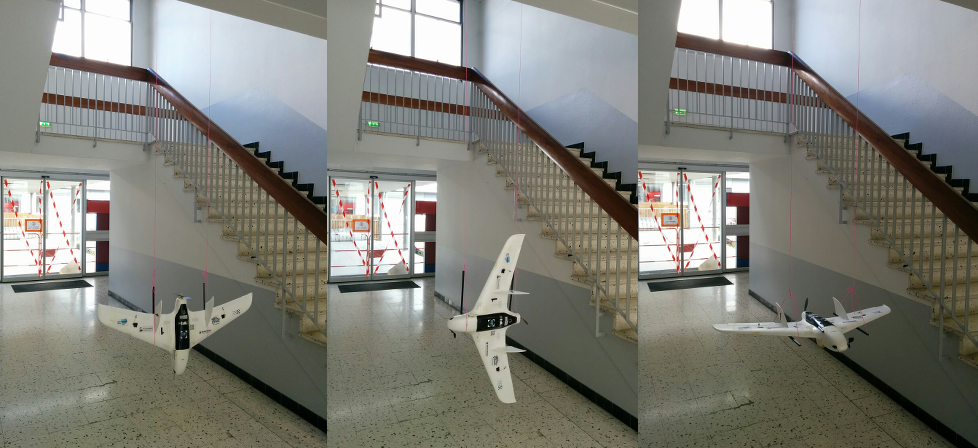
\includegraphics[width=0.9\textwidth]{figures/Mako_Inertia_combined_small.png}
      \caption{Moments of inertia measurements for each axis, $I_{xx} , I_{yy} , I_{zz} $.}
      \label{fig:inertia}
 \end{figure*}
 
 \begin{table}[!htbp]
\caption{General specifications of MAKO \cite{bronz2016aerodynamic}}
\label{arm:MAKO}
\begin{center}
\begin{tabular}{ ||p{4cm}|p{3cm}|p{2cm}||}\hline
\textbf{Parameter} & \textbf{Value} & \textbf{Definition} \\\hline
Wing span                  & $\ \ \, 1.288 $	   & $[m]$ \\\hline
Wing surface area       & $ \ \ \, 0.27 $           &  $[m^2]$ \\\hline
Mean aero chord           & $\ \ \, 0.21$           & $[m]$ \\\hline
Take-off mass              & $\ \ \, 0.7 - 2.0$       & $[kg]$ \\\hline
Flight velocity              & $\ \ \, 10 - 25$       & $[m/s]$ \\\hline
$I_{xx}$                         & $\ \ \, 0.02471284$   & $[kg \cdot m^2]$ \\\hline
$I_{yy}$                         & $\ \ \, 0.015835159$   & $[kg \cdot m^2]$ \\\hline
$I_{zz}$                         & $\ \ \, 0.037424499$   & $[kg \cdot m^2]$ \\\hline
\end{tabular}
\end{center}
\end{table}


\subsection{Attitude kinematics of aircraft}

Since the general equations of attitude motion of a rigid body, by introducing the frames of interest and angles standardized for aircraft attitude motion can be investigated next. 

Frames of interest
	ECI
	ECEF
	Navigation Frame 
	BODY

\begin{figure}
\begin{center}
%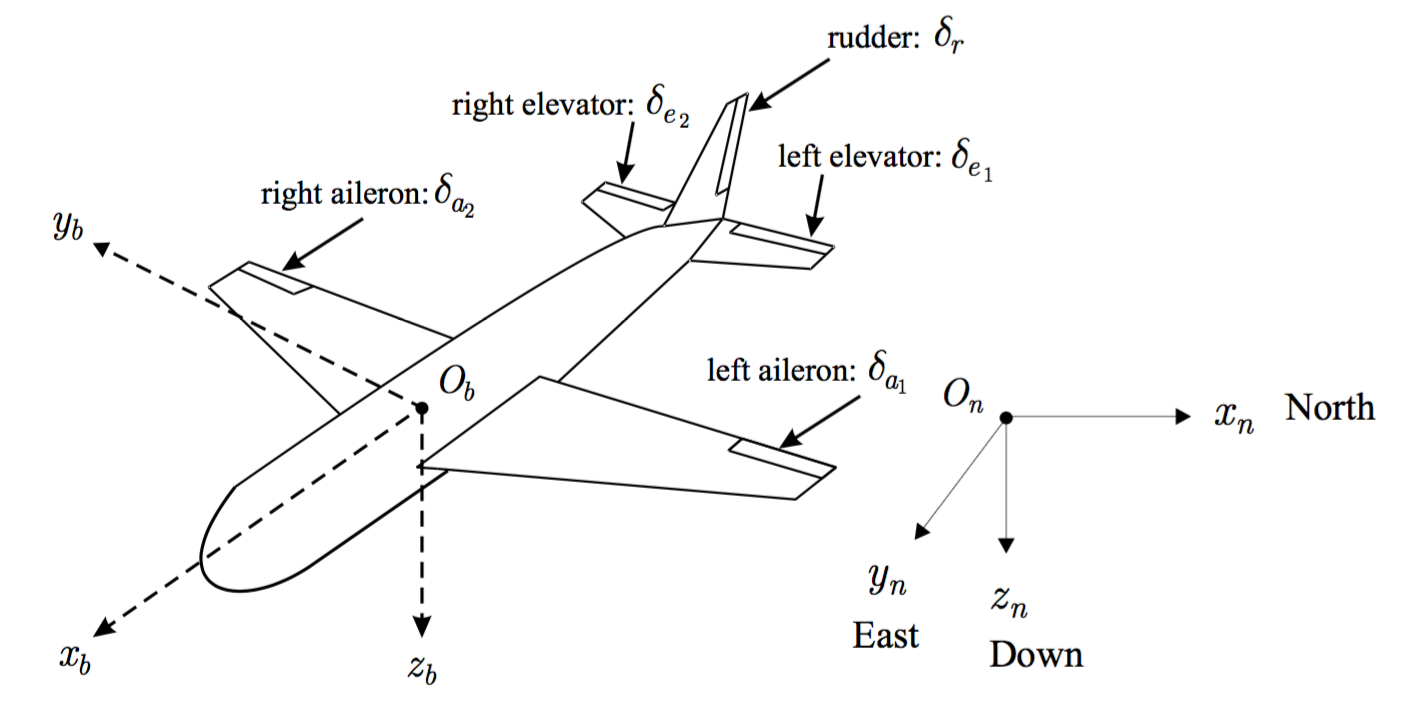
\includegraphics[width=11cm]{figures/bodyNEDframes}    % The printed column width is 8.4 cm.
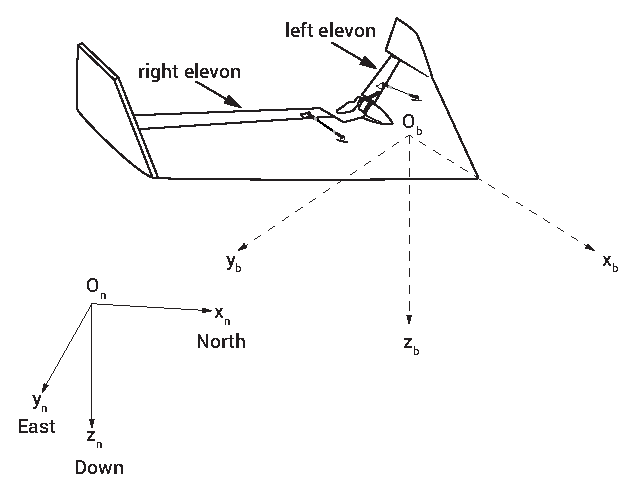
\includegraphics[width=13cm]{figures/ZagiElevon}    % The printed column width is 8.4 cm.
\caption{Body fixed frame and North East Down (NED) frame representations} 
\label{fig:bodyNEDframes}
\end{center}
\end{figure}


\begin{figure}
\begin{center}
%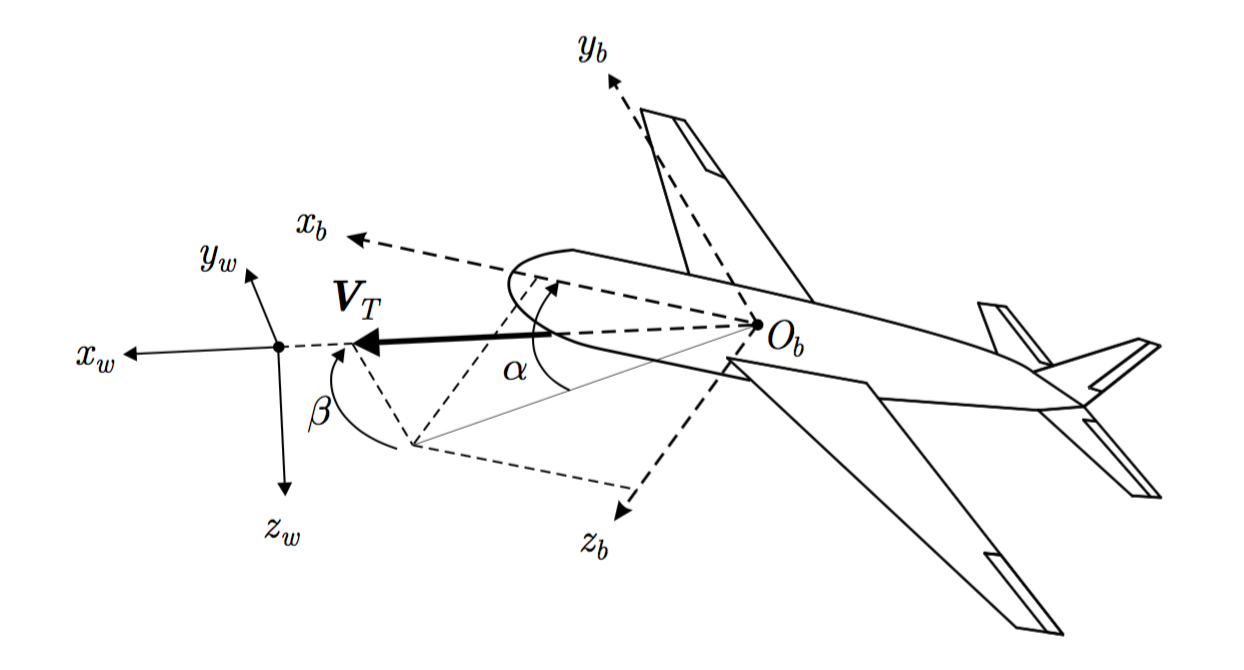
\includegraphics[width=11cm]{figures/windFrame}    % The printed column width is 8.4 cm.
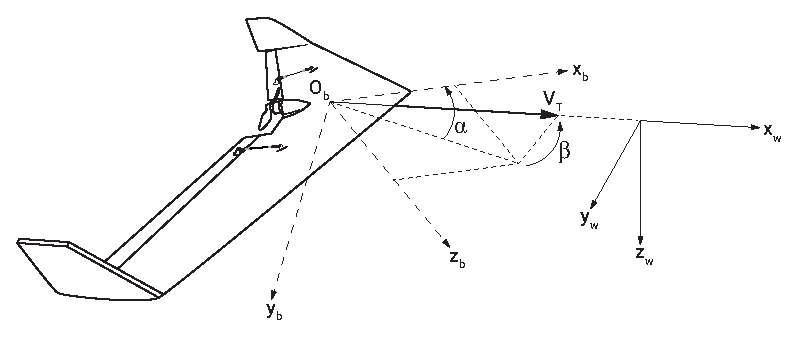
\includegraphics[width=15cm]{figures/ZagiWindframe}    % The printed column width is 8.4 cm.
\caption{Wind frame, airspeed vector $\bm{V}_T$, angle of attack $\alpha$ and side slip angle $\beta$ representation \cite{ducard2009fault}} 
\label{fig:windFrame}
\end{center}
\end{figure}

\begin{figure}
\begin{center}
%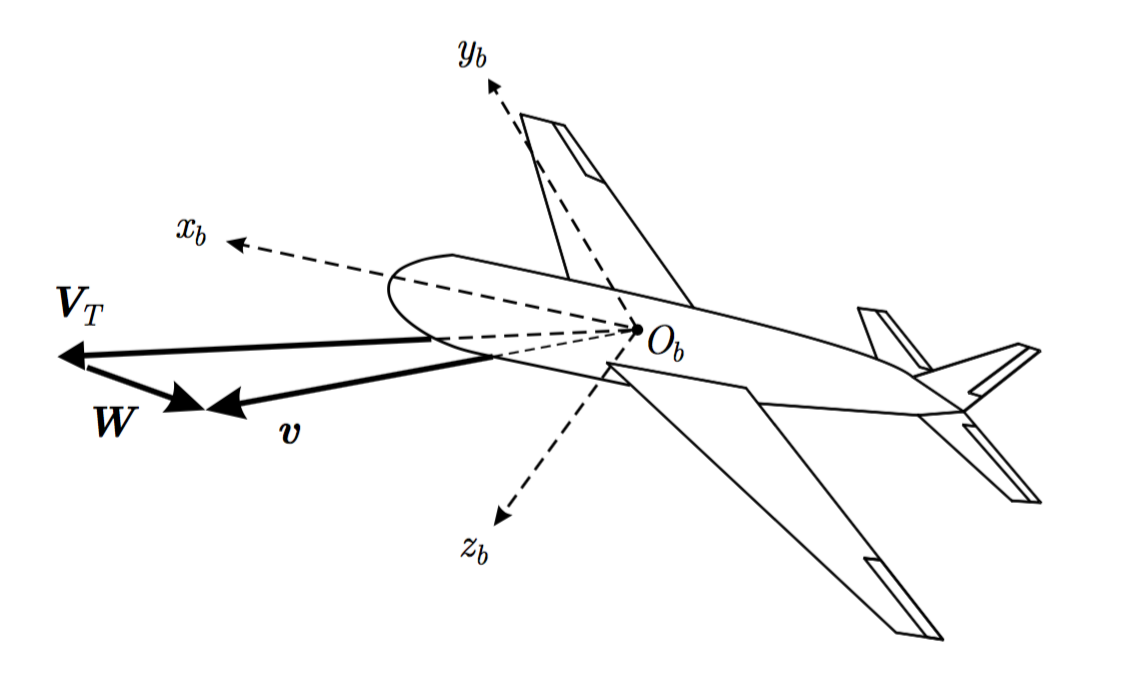
\includegraphics[width=11cm]{figures/windDisturbance}    % The printed column width is 8.4 cm.
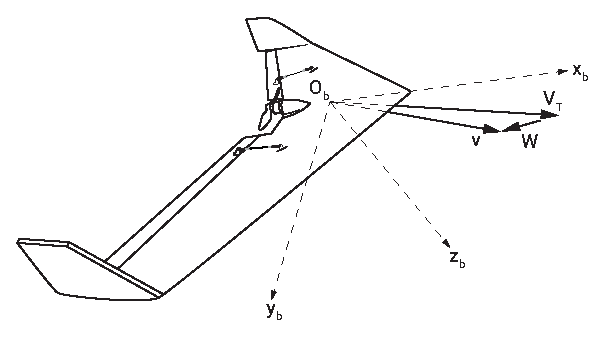
\includegraphics[width=13cm]{figures/ZagiWindDisturbance}    % The printed column width is 8.4 cm.
\caption{Relation revealed between the inertial velocity vector $\bm{v}$, airspeed vector $\bm{V}_T$ and wind disturbance $\bm{W}$ \cite{ducard2009fault}} 
\label{fig:windDisturbance}
\end{center}
\end{figure}

\begin{figure}
\begin{center}
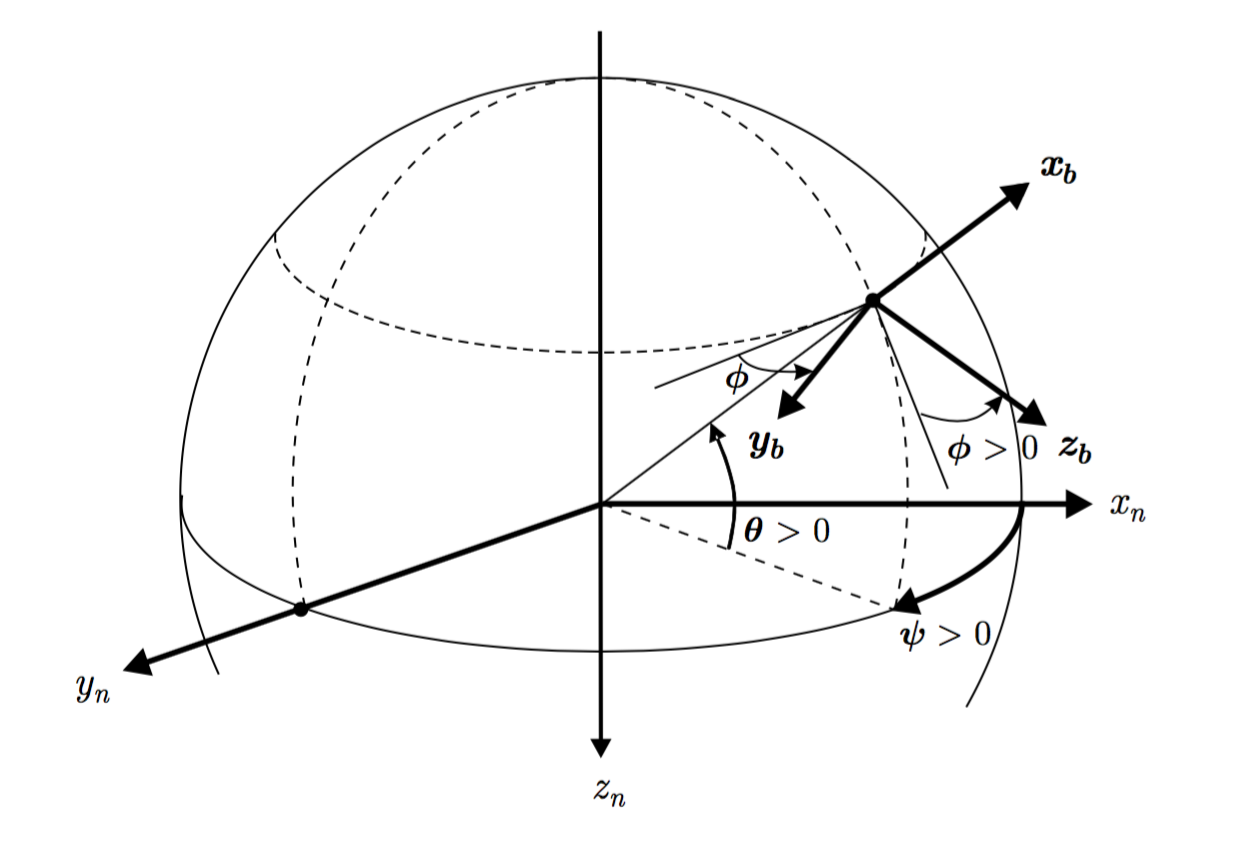
\includegraphics[width=11cm]{figures/eulerAnglesAircraft}    % The printed column width is 8.4 cm.
\caption{Euler angle sequence \cite{ducard2009fault}} 
\label{fig:eulerAnglesAircraft}
\end{center}
\end{figure}

As mentioned before, the sequence of the transformation between frames effects the final transformation matrix so does the attitude kinematics equation. In the course of the study, the sequence is assumed to be yaw - pitch - roll as is given in Fig. \ref{fig:eulerAngSequence} and the corresponding transformation matrix from the navigation frame to body-fixed frame is given in Eq. \ref{eqn:C_NtoB}.

\begin{equation}{\label{eqn:C_NtoB}}
C_N^B
= \,
\begin{bmatrix}
1 - 2(q_2^2 + q_3^2) & 2(q_1 q_2 + q_0 q_3) & 2(q_1 q_3 - q_0 q_2)  \\[0.2em]
2(q_1 q_2 - q_0 q_3) & 1 - 2(q_1^2 + q_3^2) & 2(q_2 q_3 + q_0 q_1)\\[0.2em]
2(q_1 q_3 + q_0 q_2) & 2(q_2 q_3 - q_0 q_1) & 1 - 2(q_1^2 + q_2^2) \\[0.2em]
\end{bmatrix}
\end{equation}

And finally the kinematics equation of motion for the aircraft can be written as in Eq. \ref{eqn:kinematicArrangeYPR}
\begin{equation} \label{eqn:kinematicArrangeYPR}
\begin{bmatrix}
\dot{q}_0\\[0.2em]
\dot{q}_1\\[0.2em]
\dot{q}_2\\[0.2em]
\dot{q}_3\\[0.2em]
\end{bmatrix}
 =\,
\frac{1}{2}
\,
\begin{bmatrix}
-q_1 & -q_2 & -q_3 \\
q_0 & -q_3 & q_2 \\
q_3 & q_0 & -q_1 \\
-q_2 & q_1 & q_0\\
\end{bmatrix}
\,
\begin{bmatrix}
p\\[0.2em]
q\\[0.2em]
r\\[0.2em]
\end{bmatrix} 
\end{equation}

\begin{landscape}
\begin{figure}
\begin{center}
%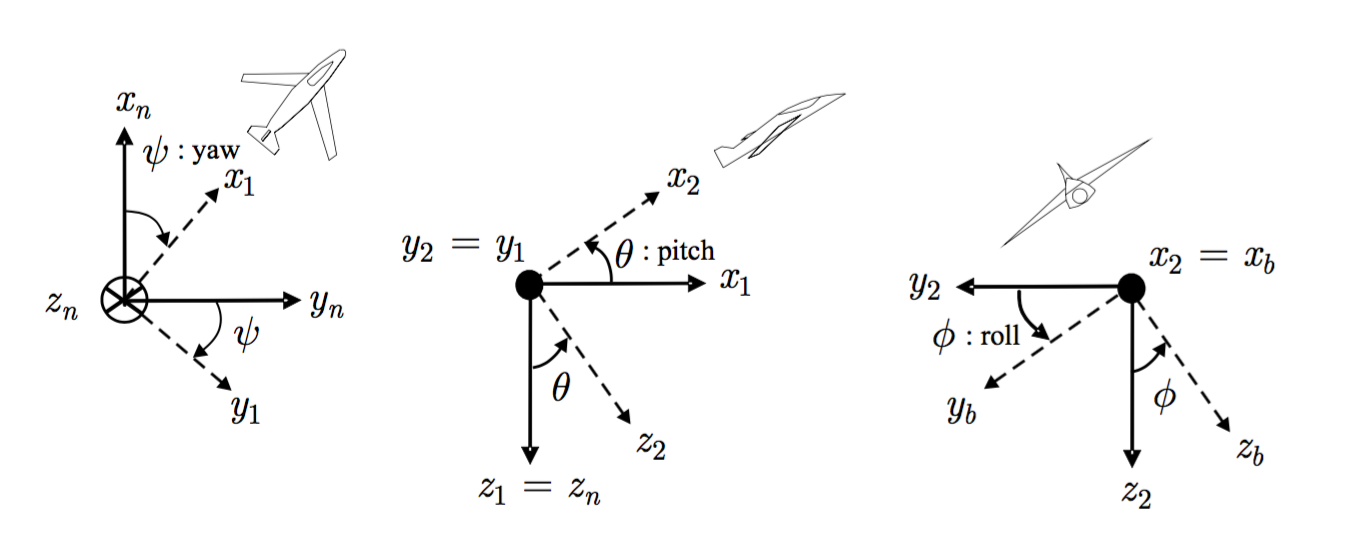
\includegraphics[width=11cm]{figures/eulerAngSequence}    % The printed column width is 8.4 cm.
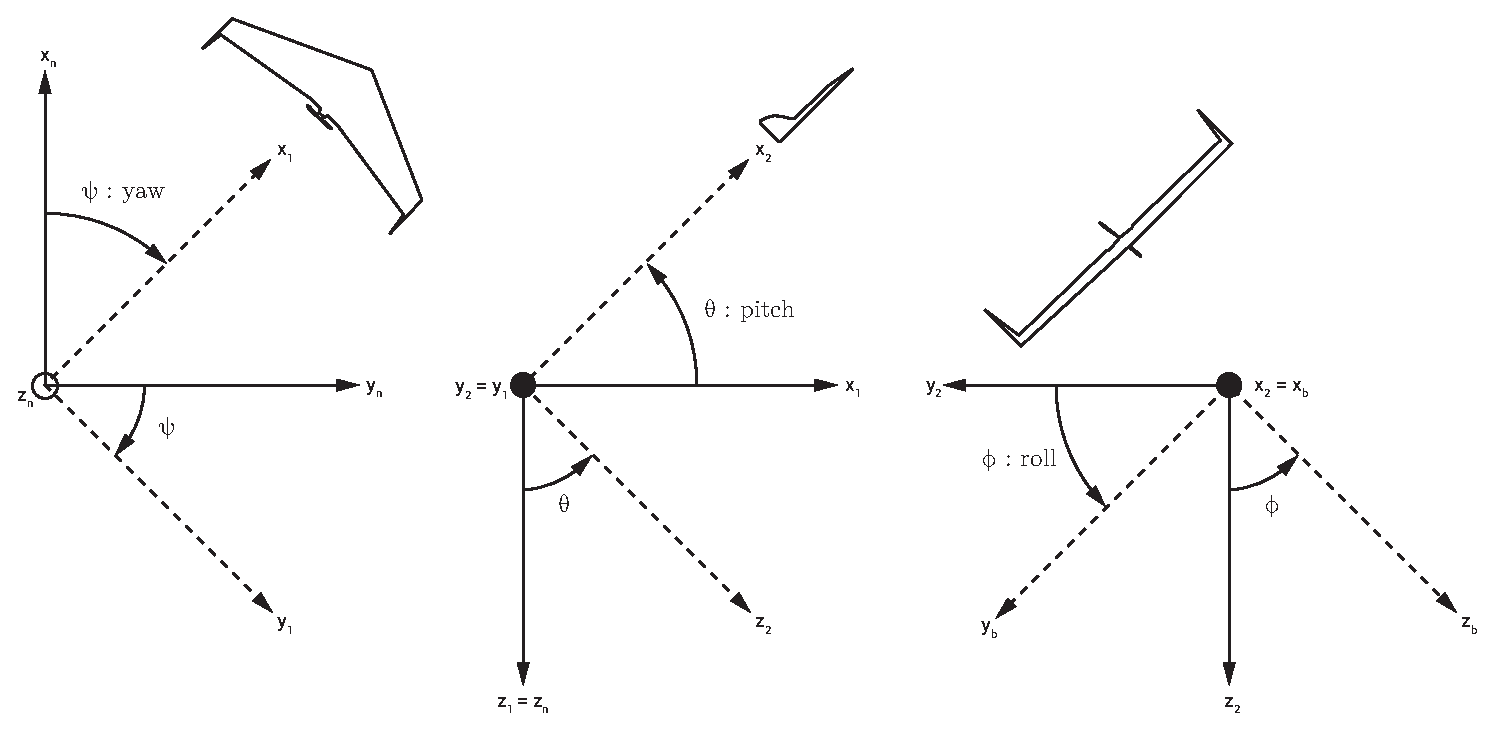
\includegraphics[width=23cm]{figures/ZagiEulerAngleSequence}
\caption{Euler angle sequence \cite{ducard2009fault}} 
\label{fig:eulerAngSequence}
\end{center}
\end{figure}
\end{landscape}

\subsection{Attitude dynamics of aircraft}

AVL is an open source program developed at MIT and uses vortex-lattice method for the aerodynamic and stability calculations.
The output of the program is linearized at a selected condition, therefore all the coefficients are calculated around the equilibrium point at $14m/s$ cruise flight condition.
The center of gravity is located at $X_{CG}= 0.295\,m$, which corresponds to a $8\,\%$ of positive static margin that has been flight tested. %FIXME we have to check if we used modified AVL with viscous add-on or not...


\subsubsection{Model of aerodynamic moments}

The attitude of the aircraft changes with the torques applied to the airframe. 

\begin{equation}{\label{eqn:torqueTotal}}
\bm{M}_B
= \,
\begin{bmatrix}
M_{Bx} \\
M_{By}\\
M_{Bz}\\
\end{bmatrix}
= \,
\begin{bmatrix}
L_{B} \\
M_{B}\\
N_{B}\\
\end{bmatrix}
\end{equation}

The torques can be given under three subclasses; roll torque $L_B$, pitch torque $M_B$, and yaw torque $N_B$.




\textbf{Roll torque}

\begin{equation}{\label{eqn:rollTorque}}
L_B = \bar{q} \, S \, b \, C_L
\end{equation}

\begin{equation}{\label{eqn:bigCraftC_L}}
C_L = C_{L_{a1}} \, \delta_{a1} + C_{L_{a2}} \, \delta_{a2} + C_{L_{e1}} \, \delta_{e1} + C_{L_{e2}} \, \delta_{e2} + C_{L_{\tilde{p}}} \, \tilde{p} + C_{L_{\tilde{r}}} \, \tilde{r} +  C_{L_\beta} \, \beta 
\end{equation}

\begin{equation}{\label{eqn:makoC_L}}
C_L = C_{L_{a}} \, \delta_{a} + C_{L_{\tilde{p}}} \, \tilde{p} + C_{L_{\tilde{r}}} \, \tilde{r} +  C_{L_\beta} \, \beta 
\end{equation}

\textbf{Pitch torque}

\begin{equation}{\label{eqn:pitchTorque}}
M_B = \bar{q} \, S \, \bar{c} \, C_M
\end{equation}

\begin{equation}{\label{eqn:bigCraftC_M}}
C_M = C_{M_{1}} + C_{M_{a1}} \, \delta_{a1} + C_{M_{a2}} \, \delta_{a2} + C_{M_{e1}} \, \delta_{e1} + C_{M_{e2}} \, \delta_{e2} + C_{M_{\tilde{q}}} \, \tilde{q} +  C_{M_\alpha} \, \alpha 
\end{equation}

\begin{equation}{\label{eqn:makoC_M}}
C_M =  C_{M_{e}} \, \delta_{e} + C_{M_{\tilde{q}}} \, \tilde{q} +  C_{M_\alpha} \, \alpha 
\end{equation}

\textbf{Yaw torque}

\begin{equation}{\label{eqn:yawTorque}}
N_B = \bar{q} \, S \, b \, C_N \\
\end{equation}


\begin{equation}{\label{eqn:bigCraftC_N}}
C_N= C_{N_{\delta r}} \, \delta_{r} + C_{N_{\tilde{r}}} \, \tilde{r} +  C_{N_\beta} \, \beta 
\end{equation}

\begin{equation}{\label{eqn:makoC_N}}
C_N= C_{N_{a}} \, \delta_{a} + C_{N_{\tilde{p}}} \, \tilde{p} + C_{N_{\tilde{r}}} \, \tilde{r} +  C_{N_\beta} \, \beta 
\end{equation}

\begin{equation}{\label{eqn:dynamicPressure}}
\bar{q} = \frac{\rho V_T^2}{2} 
\end{equation}

where $\bar{q}$ is the dynamic pressure given in  Eq. \ref{eqn:dynamicPressure}, $V_T$ is the total airspeed of the aircraft, $\rho$ is the air density, $S$ is the wing total surface, $b$ is the wing span, and $\bar{c}$ mean aerodynamic wing chord. 

\begin{table}
\label{arm:momentsETHcraft}
\caption{Stability derivatives for ETH UAV \cite{ducard2009fault}}
\label{arm:ethcraft}
\begin{center}
\begin{tabular}{ ||p{3cm}|p{3cm}|p{3cm}||}\hline
\textbf{Parameter} & \textbf{Value} & \textbf{Definition} \\\hline
$C_{L_{a1}} = - C_{L_{a2}}$ & $-3.395 \times 10^{-2}$	   & roll derivative \\\hline
$C_{L_{e1}} = - C_{L_{e2}}$ & $-0.485 \times 10^{-2}$         & roll derivative \\\hline
$C_{L_{\tilde{p}}}$                 & $-1.92 \times 10^{-1}$	   & roll derivative \\\hline
$C_{L_{\tilde{r}}} $                 & $\ \ \, 3.61 \times 10^{-2}$     & roll derivative \\\hline
$C_{L_\beta}$                        & $-1.30 \times 10^{-2}$	   & roll derivative \\\hline
$ C_{M_{1}}$                          & $\ \ \, 2.08 \times 10^{-2}$	   & pitch derivative \\\hline
$C_{M_{a1}} = C_{M_{a2}} $ & $\ \ \, 0.389 \times 10^{-1}$  & pitch derivative \\\hline
$C_{M_{e1}} = C_{M_{e2}} $ & $\ \ \, 2.725 \times 10^{-1}$  &  pitch derivative \\\hline
$C_{M_{\tilde{q}}} $               & $-9.83$	                            & pitch derivative \\\hline
$C_{M_\alpha} $                    & $-9.03 \times 10^{-2}$ 	   & pitch derivative \\\hline
$C_{N_{\delta r}}$                  & $\ \ \, 5.34 \times 10^{-2}$ 	   & yaw derivative \\\hline
$ C_{N_{\tilde{r}}}$                 & $-2.14 \times 10^{-1}$	   & yaw derivative \\\hline
$C_{N_\beta} $                       & $\ \ \, 8.67 \times 10^{-2}$	     & yaw derivative \\\hline
\end{tabular}
\end{center}
\end{table}

\begin{table}
\label{arm:momentsMAKO}
\caption{Stability derivatives for MAKO extracted from AVL program at $14 m/s$ equilibrium cruise speed \cite{bronz2016aerodynamic}}
\label{arm:MAKO}
\begin{center}
\begin{tabular}{ ||p{3cm}|p{3cm}|p{3cm}||}\hline
\textbf{Parameter} & \textbf{Value} & \textbf{Definition} \\\hline
$C_{L_a}$                             & $-0.1956 \times 10^{-2}$	   & roll derivative \\\hline
$C_{L_{\tilde{p}}}$                 & $-4.095 \times 10^{-1}$	   & roll derivative \\\hline
$C_{L_{\tilde{r}}} $                 & $\ \ \, 6.203 \times 10^{-2}$     & roll derivative \\\hline
$C_{L_\beta}$                        & $\ \ \, 3.319 \times 10^{-2}$	   & roll derivative \\\hline
$C_{M_0}$ 			     & $\ \ \, 0$  &  pitch derivative \\\hline
$C_{M_e}$ 			     & $-0.076 \times 10^{-1}$  &  pitch derivative \\\hline
$C_{M_{\tilde{q}}} $               & $-1.6834$	                            & pitch derivative \\\hline
$C_{M_\alpha} $                    & $-32.34 \times 10^{-2}$ 	   & pitch derivative \\\hline
$C_{N_a}$                             & $-0.0126 \times 10^{-2}$	   & yaw derivative \\\hline
$C_{N_{\tilde{p}}}$                 & $-4.139 \times 10^{-2}$ 	   & yaw derivative \\\hline
$C_{N_{\tilde{r}}}$                 & $-0.1002 \times 10^{-1}$	   & yaw derivative \\\hline
$C_{N_\beta} $                      & $\ \ \, 2.28 \times 10^{-2}$	   & yaw derivative \\\hline
\end{tabular}
\end{center}
\end{table}


%%%%%%%%%%%%%%%%%% FORCE CALCULATIONS


%%%% LIFT FORCE %%%%

\textbf{Lift force}

\begin{equation}{\label{eqn:liftForce}}
Z^w = \bar{q} \, S \,  C_Z(\alpha)
\end{equation}

\begin{equation}{\label{eqn:dynamicPressure}}
\bar{q} = \frac{\rho V_T^2}{2} 
\end{equation}

\begin{equation}{\label{eqn:liftCoef}}
C_Z(\alpha) = C_{Z_0} + C_{Z_{\alpha}} \alpha 
\end{equation}


%%%% DRAG FORCE %%%%

\textbf{Drag force}

\begin{equation}{\label{eqn:dragForceETHcraft}}
X^w = \bar{q} \, S \,  C_X(\alpha, \beta)
\end{equation}

\begin{equation}{\label{eqn:dragCoeffETHcraft}}
C_X(\alpha, \beta) = C_{X_1} + C_{X_{\alpha}} \alpha + C_{X_{\alpha 2}} {\alpha}^2 + C_{X_{\beta 2}} {\beta}^2 
\end{equation}

\begin{equation}{\label{eqn:dragForceMAKO}}
X^w = \bar{q} \, S \, C_{Z}(\alpha, \beta)
\end{equation}

\begin{equation}{\label{eqn:dragCoeffMAKO}}
C_X(\alpha) = C_{X_1} + C_{X_k} \, C_Z^2 = C_{X_1} + C_{X_k} \, (C_{Z_1} + C_{Z_{\alpha}} \alpha )^2
\end{equation}

%%%% LATERAL FORCE %%%%

\textbf{Lateral force}

\begin{equation}{\label{eqn:lateralForceETHcraft}}
Y^w = \bar{q} \, S \,  C_Y(\beta)
\end{equation}

\begin{equation}{\label{eqn:lateralCoeffETHcraft}}
C_Y(\beta) = C_{Y_\beta} \beta
\end{equation}

\begin{equation}{\label{eqn:lateralCoeffMAKO}}
C_Y(\beta, \, \tilde{p}, \, \tilde{r}, \, \delta_a) = C_{Y_\beta} \beta + C_{Y_{\tilde{p}}} \, \tilde{p} + C_{Y_{\tilde{r}}} \, \tilde{r} + C_{Y_a} \, \delta_a 
\end{equation}

\begin{table}
\label{arm:forcesETHcraft}
\caption{Aerodynamic force derivatives for ETH UAV \cite{ducard2009fault}}
\label{arm:ethcraft}
\begin{center}
\begin{tabular}{ ||p{3cm}|p{3cm}|p{4cm}||}\hline
\textbf{Parameter} & \textbf{Value} & \textbf{Definition} \\\hline
$C_{Z_0}$                             & $\ \ \,1.29 \times 10^{-2}$	   & lift derivative \\\hline
$C_{Z_{\alpha}}$                   & $-3.25 $                                 & lift derivative \\\hline
$C_{X_1}$                             & $-2.12 \times 10^{-2}$	   & drag derivative \\\hline
$C_{X_{\alpha}}$                   & $-2.66 \times 10^{-2}$          & drag derivative \\\hline
$C_{X_{\alpha 2}}$                & $-1.55 $	                            & drag derivative \\\hline
$C_{X_{\beta 2}} $                 & $-4.01 \times 10^{-1}$	   & drag derivative \\\hline
$C_{Y_\beta} $                      & $-3.79 \times 10^{-1}$          & side force derivative \\\hline
\end{tabular}
\end{center}
\end{table}


\begin{table}
\label{arm:forcesMAKO}
\caption{Aerodynamic force derivatives for MAKO extracted from AVL program at $14 m/s$ equilibrium cruise speed \cite{bronz2016aerodynamic}}
\label{arm:MAKO}
\begin{center}
\begin{tabular}{ ||p{3cm}|p{3cm}|p{4cm}||}\hline
\textbf{Parameter} & \textbf{Value} & \textbf{Definition} \\\hline
$C_{Z_0}$                             & $-8.53 \times 10^{-2}$	         & lift derivative \\\hline
$C_{Z_{\alpha}}$                   & $\ \ \,3.9444$                               & lift derivative \\\hline
$C_{Z_q}$                             & $\ \ \,4.8198$	       		         & lift derivative \\\hline
$C_{Z_e}$                             & $\ \ \,1.6558 \times 10^{-2}$        & lift derivative \\\hline
$C_{X_0}$                             & $\ \ \, 2.313 \times 10^{-2}$	   & drag derivative \\\hline
$C_{X_k}$                              & $\ \ \, 1.897 \times 10^{-1}$          & drag derivative \\\hline
$C_{Y_\beta}$ 			     & $-2.708 \times 10^{-1}$             & side force derivative \\\hline
$C_{Y_{\tilde{p}}}$                 & $\ \ \, 1.695 \times 10^{-2}$	& side force derivative \\\hline
$C_{Y_{\tilde{r}}}$                  & $\ \ \, 5.003 \times 10^{-2}$ 	& side force derivative \\\hline
$C_{Y_a}$                             & $\ \ \, 0.0254 \times 10^{-2}$	& side force derivative \\\hline
\end{tabular}
\end{center}
\end{table}

%%%% THRUST FORCE %%%%

\subsubsection{Thrust force model}

\begin{equation}{\label{eqn:thrustModel}}
F_T = \rho n^2 D^4 C_{F_T}
\end{equation}

\begin{equation}{\label{eqn:thrustETHcraft}}
C_{F_T} = C_{F_{T1}} + C_{F_{T2}} J + C_{F_{T3}} J^2 
\end{equation}

\begin{equation}{\label{eqn:advRatETHcraft}}
J = \frac{V_T}{n \pi D}
\end{equation}

\begin{table}
\label{arm:ETHcraft}
\caption{Thrust force coefficients for propeller ETH UAV \cite{ducard2009fault}}
\label{arm:thrustForce}
\begin{center}
\begin{tabular}{ ||p{3cm}|p{3cm}|p{4cm}||}\hline
\textbf{Parameter} & \textbf{Value} & \textbf{Definition} \\\hline
$C_{F_{T1}} $                 & $\ \ \, 8.42 \times 10^{-2}$	   & thrust derivative \\\hline
$C_{F_{T2}} $                 & $-1.36 \times 10^{-1}$	           & thrust derivative \\\hline
$C_{F_{T3}} $                 & $-9.28 \times 10^{-1}$                 & thrust derivative \\\hline
$D$                                 & $\ \ \, 0.79 \, m$                           & propeller diameter \\\hline
\end{tabular}
\end{center}
\end{table}

\begin{equation}{\label{eqn:thrustCoefMAKO}}
C_{F_T} = C_{F_{T1}} + C_{F_{T2}} J^\prime + C_{F_{T_{rpm}}} \frac{n}{60} 
\end{equation}

\begin{equation}{\label{eqn:advRatMAKO}}
J^\prime = \frac{V_T}{n D}
\end{equation}

\begin{table}
\label{arm:MAKO}
\caption{Thrust force coefficients for propeller APC SF $9 \times 6$ from wind tunnel experiments \cite{bronz2017flight}}
\label{arm:thrustForce}
\begin{center}
\begin{tabular}{ ||p{3cm}|p{3cm}|p{4cm}||}\hline
\textbf{Parameter} & \textbf{Value} & \textbf{Definition} \\\hline
$C_{F_{T1}}$                   & $\ \ \, 1.342 \times 10^{-1}$	   & thrust derivative \\\hline
$C_{F_{T2}}$                 & $-1.975 \times 10^{-1}$	          & thrust derivative \\\hline
$C_{F_{T_{rpm}}}  $           & $\ \ \, 7.048 \times 10^{-6}$    & thrust derivative \\\hline
$D$                              & $\ \ \, 0.228 \, m$                          & propeller diameter \\\hline
\end{tabular}
\end{center}
\end{table}

\section{Shortcut to modeling}

Nonlinear aircraft flight dynamics for translational and attitude motion can be given as a system of first order differential equations 

\begin{align}{\label{eqn:compactEquOfMotion}}
\begin{split}
\dot{\bm{x}}_{n} &= \bm{C}_b^n \bm{v}^b\\
\dot{\bm{v}}^b &= \frac{1}{m} \big[ m \bm{g}^b + \bm{F}_t^b + \bm{F}_a^b \big] - {\bm{\omega}_{b/n}^b}^\times \bm{v}^b  \\
\dot{q}_0 &= -\frac{1}{2} \bm{q}_\nu^T \bm{\omega}_{b/n}^b\\
\dot{\bm{q}}_\nu &= \frac{1}{2}\Big(\bm{q}_\nu^\times + q_0 \bm{I}_3 \Big) \bm{\omega}_{b/n}^b \\
\bm{J} \dot{\bm{\omega}}_{b/n}^b &= \bm{M} - {\bm{\omega}_{b/n}^b}^\times \bm{J} \bm{\omega}_{b/n}^b\\
\end{split}
\end{align}

where $\bm{x}_{n} \in {\rm I\!R^3}  $ is the position of the center of mass of UAV in navigation frame $\mathcal{N}$, $\bm{v}^b$ is the velocity of the center of mass of UAV in body frame $\mathcal{B}$,  $\bm{q} = [q_0, \bm{q}_v^T] ^T \in {\rm I\!R^3} \times {\rm I\!R}$ is the unit quaternion representing the attitude of the body frame $\mathcal{B}$ with respect to navigation frame $\mathcal{N}$ expressed in the body frame $\mathcal{B}$, $\bm{\omega}_{b/n}^b$ is the angular velocity of the body frame $\mathcal{B}$ with respect to navigation frame $\mathcal{N}$ expressed in the body frame $\mathcal{B}$, $ \bm{J} \in {\rm I\!R^{3\times3}}  $ is the positive definite inertia matrix of the drone, $\bm{M} \in {\rm I\!R^3}$ represents the moments acting on the drone, $ \bm{C}_b^n$ is the direction cosine matrix which transforms a vector expressed in the body frame to its equal expressed in the navigation frame, $\bm{I}_3  \in {\rm I\!R^{3\times3}}$ is the identity matrix, $\bm{F}_t^b \in {\rm I\!R^3}$ is the thrust force expressed in the body frame,  $\bm{F}_a^b \in {\rm I\!R^3}$ are the aerodynamic forces given in the body frame. 
The navigation frame is assumed to be a local inertial frame in which Newton's Laws apply. 
The notation $\bm{x} ^{\times} $ for a vector $x = [x_1 \quad x_2 \quad x_3]^ {\rm{T}}$ represents the skew-symmetric matrix

\begin{equation}
\bm{x} ^ \times= \begin{bmatrix} 
0 & -x_3 & x_2 \\
x_3 & 0 & -x_1 \\
-x_2 & x_1 & 0 \\
 \end{bmatrix}
\end{equation}


\begin{align}{\label{eqn:aeroMoments}}
\begin{split}
L& = \bar{q} \, S \, b \, C_L \\
M& = \bar{q} \, S \, \bar{c} \, C_M \\
N& = \bar{q} \, S \, b \, C_N \\
\end{split}
\end{align}

\section{Verification with Matlab Simulink 6DOF block}

To validate the written translational and attitude motion dynamics and kinematics, MATLAB Simulink \textit{6DOF} block has been utilized.
This block accepts inputs as the force and moment and outputs the states of aircraft motion Fig.~\ref{figure:validationSimulink}.
To compare the generated model and Simulink \textit{6DOF} block, forces and moments have been calculated via equations and constants given in Appendix A and Appendix B.
The simulated states from the model script have been saved in advance and called from Simulink by \textit{From Workspace} blocks then compared with the \textit{6DOF} outputs.
The difference found to be negligible indicating the validity of the model. 


\begin{figure*}
\center
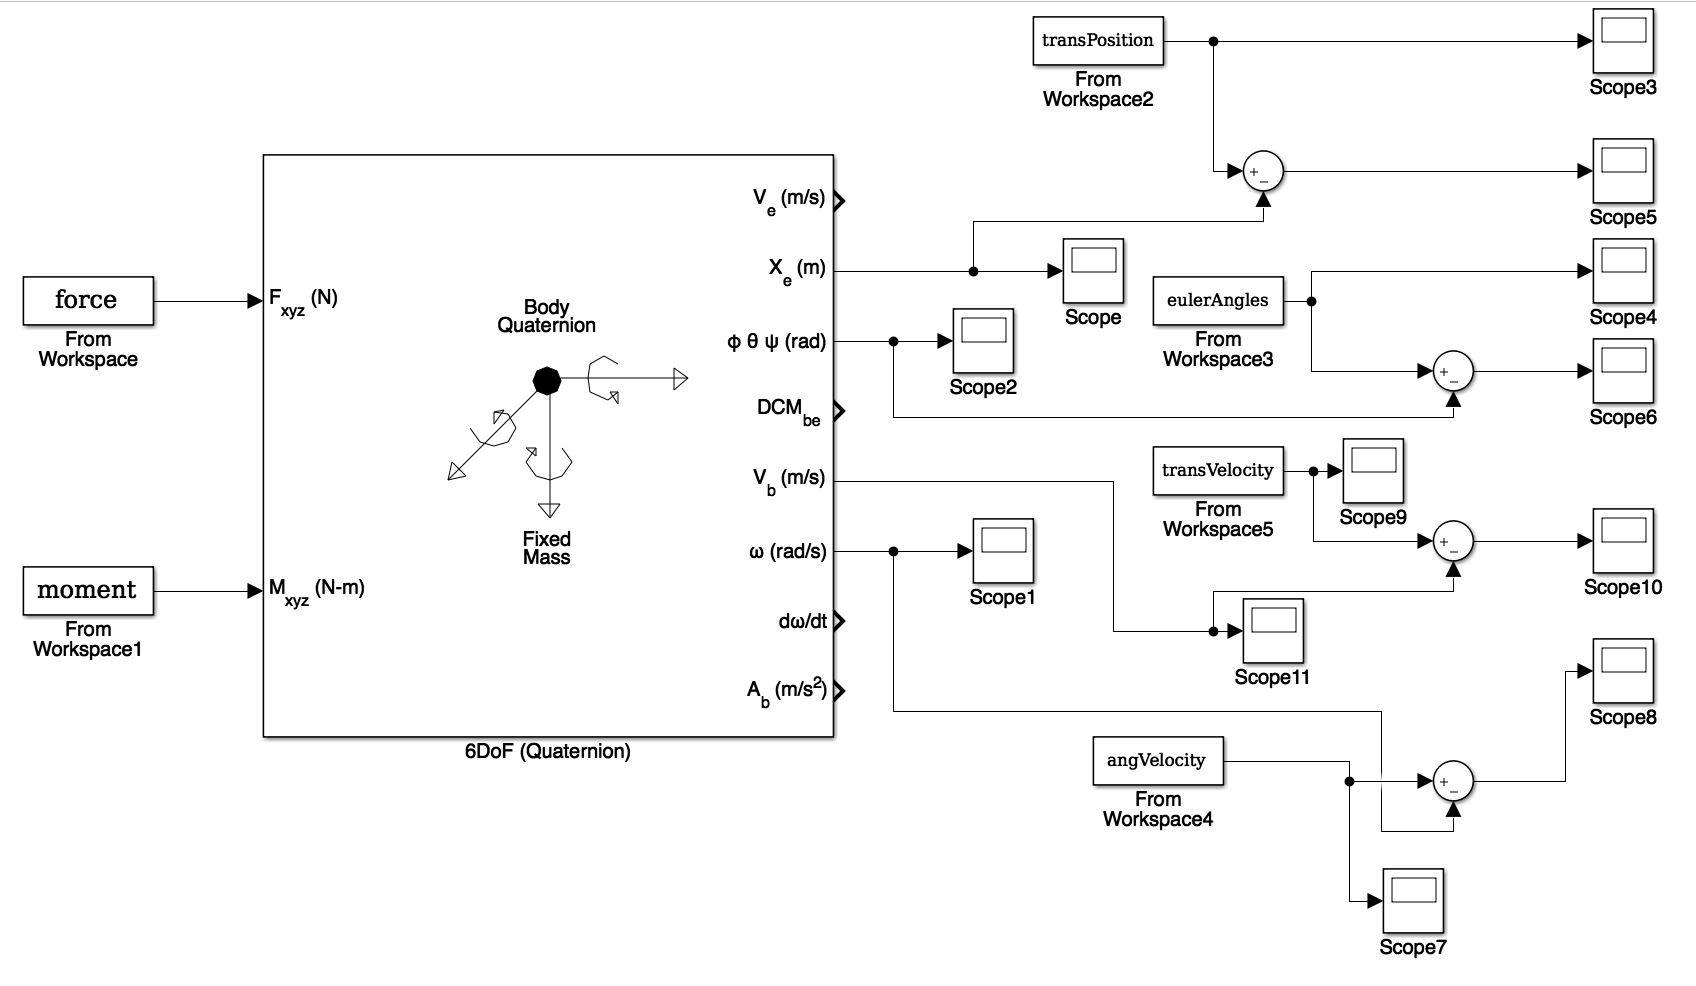
\includegraphics[width=1.1\columnwidth]{figures/validationViaSimulink}
\caption{Validation with Simulink 6DOF aircraft model}
\label{figure:validationSimulink}
\end{figure*}


\section{Sensor Models}

The measurements are simulated using the statistics of the hardware in the house.
The sensor suit simulated is the InvenSense MPU-9250 Nine-axis (Gyro + Accelerometer + Compass) MEMS MotionTracking Device. 
 
 \begin{align}
\bm{z}_{gyro} &= \bm{k}_{gyro} \bm{\omega}_{b/i}^b + \bm{\beta}_{gyro} + \bm{\eta}_{gyro}\\
\bm{z}_{acc} &= \bm{k}_{acc} \bm{\omega}_{b/i}^b + \bm{\beta}_{acc} + \bm{\eta}_{acc}
% hic bir sey yazmazsan esitlikleri alt alta hizaliyor canim benim&=alo \\
% $ tek dolar arasi $ inline denklem
% $$ cift dolar arasi $$ satir atlayarak ortada denklem
\end{align}

\begin{table}[!htbp]
\caption{Specifications of the sensor suit InvenSense MPU-9250 Nine-axis (Gyro + Accelerometer + Compass) MEMS MotionTracking Device\cite{condomines2015developpement}}
\label{arm:sensorSpecs}
\begin{center}
\begin{tabular}{ ||p{3cm}|p{2cm}|p{1.5cm}||}\hline
\textbf{Measurement} & $ \bm{\beta}$ &  $ \bm{\sigma}$ \\\hline
${\bm{z}_{acc}}_x$                  & $\ \ \, 0.142 $	   & $\ \ \, 0.0319$ \\\hline
${\bm{z}_{acc}}_y$       & $ -0.3 $           &  $\ \ \, 0.0985$ \\\hline
${\bm{z}_{acc}}_z$           & $\ \ \, 0.19$           & $\ \ \, 0.049$ \\\hline
${\bm{z}_{gyro}}_x$                  & $-1.55 $	   & $\ \ \, 0.0825$ \\\hline
${\bm{z}_{gyro}}_y$       & $ -1.13 $           &  $\ \ \, 0.1673$ \\\hline
${\bm{z}_{gyro}}_z$           & $-1.7$           & $\ \ \, 0.2214$ \\\hline
\end{tabular}
\end{center}
\end{table}

Here $\bm{\beta}$ is the bias, and $\bm{\eta}$ is the zero mean Gaussian process with $\bm{\sigma}^2$ variance and given in Table ~\ref{arm:sensorSpecs}.


\section{Fault Models}

\begin{equation}
\bm{u}\left(t\right)= \begin{bmatrix} {\delta}_{a}\ {\delta}_{e}\ n \end{bmatrix}^{\rm T}
\end{equation}

Here $ \delta_{a}$ aileron deflection angle in degrees, $ \delta_{e}$ elevator deflection angle in degrees, $n$ engine speed in rev/s. 


When the actuators are healthy, actual control input signal will be equal to the given input signal.
In case of a fault the actual signal can be modeled as

\begin{equation}
\bm{u}\left(t\right)= \bm{E}\bm{u}_c + \bm{u}_f
\end{equation}

where $\bm{u}_c $ is the desired control signal, $\bm{E} = diag(e_1, e_2, e_3)$ is the effectiveness of the actuators where $0 \leq e_i \leq 1 $ with $(i = 1, 2 ,3)$ and $\bm{u_f}$ additive actuator fault. This model makes it possible to simulate all four types of actuator faults shown in Fig.~\ref{fig:actuatorFaults}.


\begin{figure}
\begin{center}
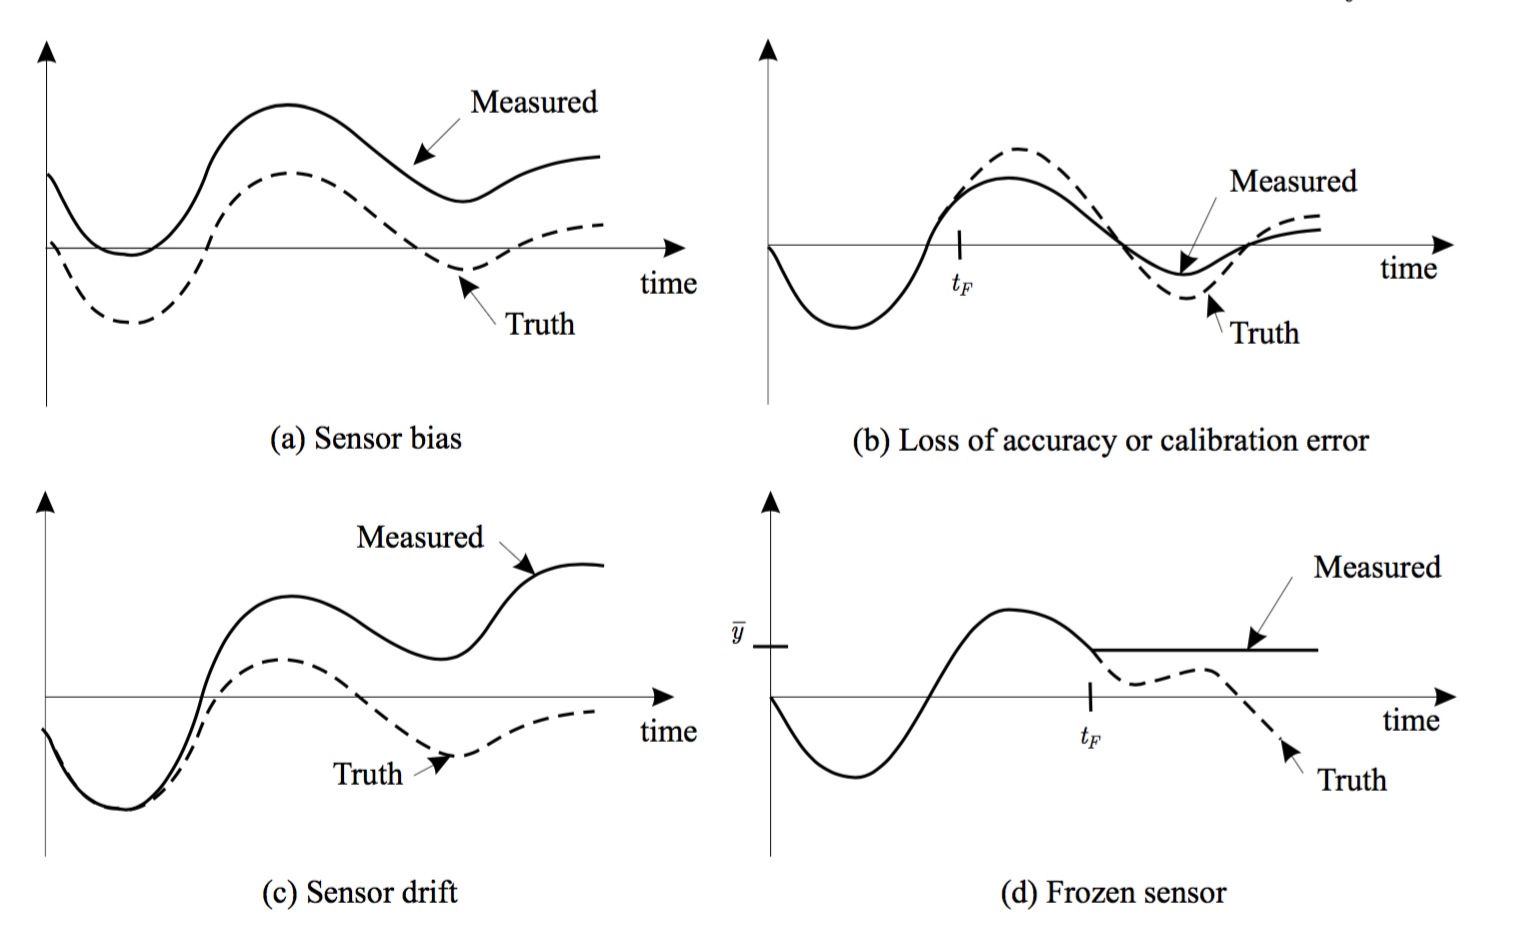
\includegraphics[width=11cm]{figures/sensorFaults}    % The printed column width is 8.4 cm.
\caption{Probable sensor faults \cite{ducard2009fault}} 
\label{fig:sensorFaults}
\end{center}
\end{figure}

\begin{figure}
\begin{center}
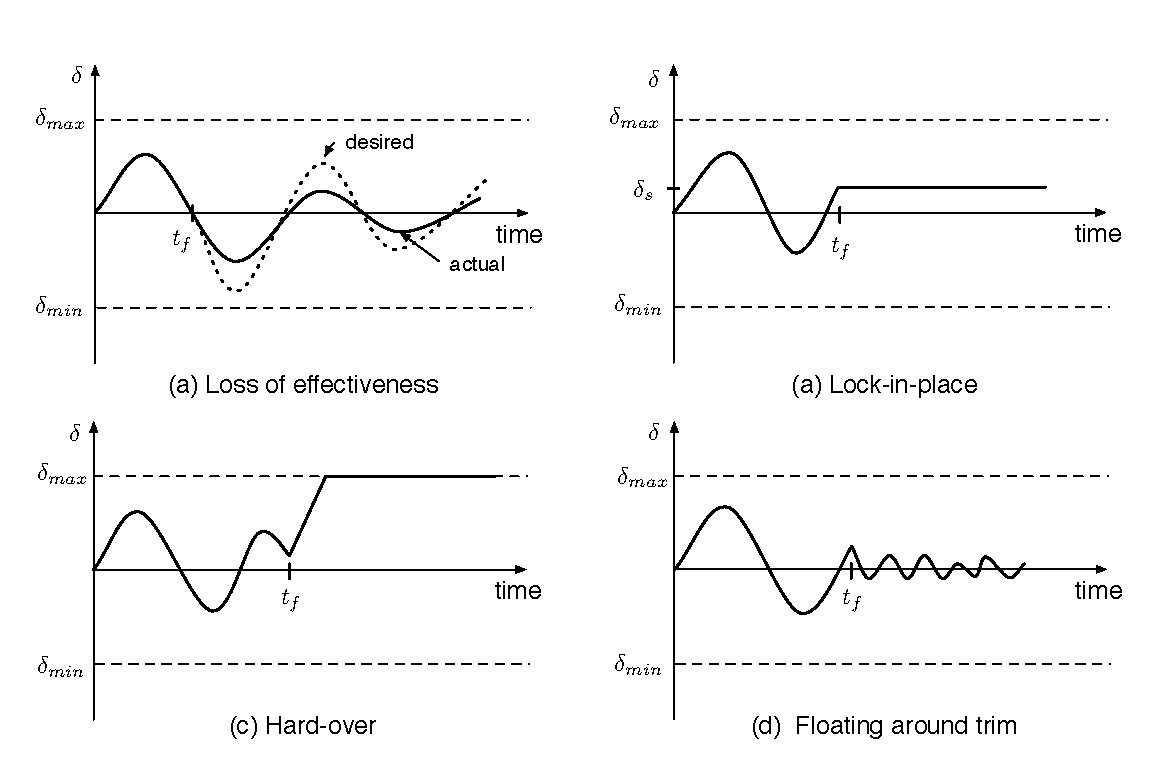
\includegraphics[width=13cm]{figures/actuatorFaults}    % The printed column width is 8.4 cm.
\caption{Probable actuator faults \cite{ducard2009fault}} 
\label{fig:actuatorFaults}
\end{center}
\end{figure}




%\begin{equation}
%\bm{\dot{x}}\left(t\right) = \bm{f}\left(\bm{x}\left(t\right) , \bm{u}\left(t\right) \right) 
%\end{equation}


%\begin{align}
%{{\mu }_{nf}}\frac{{{\partial }^{2}}u}{\partial {{y}^{2}}}+{{\left( \rho \beta  \right)}_{nf}}g\sin \phi \left( T-{{T}_{w2}} \right)-{{\sigma }_{nf}}B_{0}^{2} \sin^{2}\left( \alpha + \phi \right) u&=\frac{\partial p}{\partial x}  \label{equ1} \\
%\frac{{{\partial }^{2}}T}{\partial {{y}^{2}}}+\frac{{{\mu }_{nf}}}{{{k}_{nf}}}{{\left( \frac{\partial u}{\partial y} \right)}^{2}}+\frac{{{\sigma }_{nf}}}{{{k}_{nf}}}B_{0}^{2} \sin^{2}\left( \alpha + \phi \right){{u}^{2}}&=0 \label{equ2} \ 
% hic bir sey yazmazsan esitlikleri alt alta hizaliyor canim benim&=alo \\
% $ tek dolar arasi $ inline denklem
% $$ cift dolar arasi $$ satir atlayarak ortada denklem
%\end{align}
%%%%% End of Eq 1 & Eq 2 %%%%%
%The system of equations in  Eq (1-2) is subject to boundary conditions given in (3-4)
%%%%%% Eq 3 & Eq 4 %%%%%%
%\begin{align}
%u(H / 2)&=0   & u(-H / 2)&=0\\
%T(H / 2)&= {T}_{w1} & T(- H / 2)&= {T}_{w2}0
%\end{align}

%\begin{figure}
%\begin{center}
%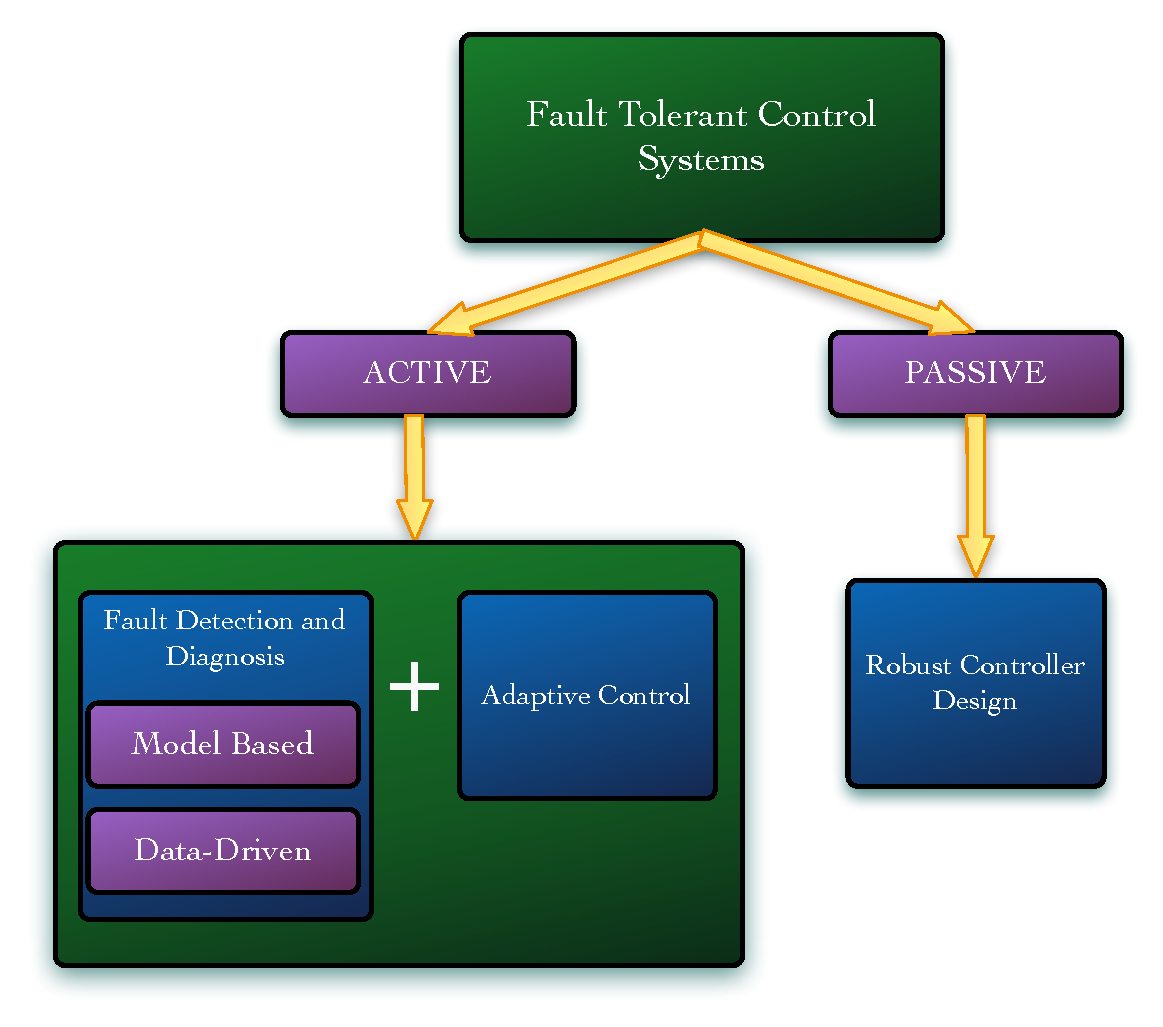
\includegraphics[width=8.3cm]{FTCmethods}    % The printed column width is 8.4 cm.
%\caption{Variations of fault tolerant control systems } 
%\label{fig:FTCmethods}
%\end{center}
%\end{figure}

%\begin{table}
%\caption{Attitude representations comparison}
%\label{tab:attRepSelection}
%\begin{center}
%\begin{tabular}{||l|l||}\hline
%Representation & Number of parameter set & Properties \\\hline
%our	   & friends \\\hline
%\end{tabular}
%\end{center}
%\end{table}






